% Options for packages loaded elsewhere
\PassOptionsToPackage{unicode}{hyperref}
\PassOptionsToPackage{hyphens}{url}
\PassOptionsToPackage{dvipsnames,svgnames,x11names}{xcolor}
%
\documentclass[
  letterpaper,
  DIV=11,
  numbers=noendperiod]{scrreprt}

\usepackage{amsmath,amssymb}
\usepackage{iftex}
\ifPDFTeX
  \usepackage[T1]{fontenc}
  \usepackage[utf8]{inputenc}
  \usepackage{textcomp} % provide euro and other symbols
\else % if luatex or xetex
  \usepackage{unicode-math}
  \defaultfontfeatures{Scale=MatchLowercase}
  \defaultfontfeatures[\rmfamily]{Ligatures=TeX,Scale=1}
\fi
\usepackage{lmodern}
\ifPDFTeX\else  
    % xetex/luatex font selection
\fi
% Use upquote if available, for straight quotes in verbatim environments
\IfFileExists{upquote.sty}{\usepackage{upquote}}{}
\IfFileExists{microtype.sty}{% use microtype if available
  \usepackage[]{microtype}
  \UseMicrotypeSet[protrusion]{basicmath} % disable protrusion for tt fonts
}{}
\makeatletter
\@ifundefined{KOMAClassName}{% if non-KOMA class
  \IfFileExists{parskip.sty}{%
    \usepackage{parskip}
  }{% else
    \setlength{\parindent}{0pt}
    \setlength{\parskip}{6pt plus 2pt minus 1pt}}
}{% if KOMA class
  \KOMAoptions{parskip=half}}
\makeatother
\usepackage{xcolor}
\setlength{\emergencystretch}{3em} % prevent overfull lines
\setcounter{secnumdepth}{5}
% Make \paragraph and \subparagraph free-standing
\makeatletter
\ifx\paragraph\undefined\else
  \let\oldparagraph\paragraph
  \renewcommand{\paragraph}{
    \@ifstar
      \xxxParagraphStar
      \xxxParagraphNoStar
  }
  \newcommand{\xxxParagraphStar}[1]{\oldparagraph*{#1}\mbox{}}
  \newcommand{\xxxParagraphNoStar}[1]{\oldparagraph{#1}\mbox{}}
\fi
\ifx\subparagraph\undefined\else
  \let\oldsubparagraph\subparagraph
  \renewcommand{\subparagraph}{
    \@ifstar
      \xxxSubParagraphStar
      \xxxSubParagraphNoStar
  }
  \newcommand{\xxxSubParagraphStar}[1]{\oldsubparagraph*{#1}\mbox{}}
  \newcommand{\xxxSubParagraphNoStar}[1]{\oldsubparagraph{#1}\mbox{}}
\fi
\makeatother

\usepackage{color}
\usepackage{fancyvrb}
\newcommand{\VerbBar}{|}
\newcommand{\VERB}{\Verb[commandchars=\\\{\}]}
\DefineVerbatimEnvironment{Highlighting}{Verbatim}{commandchars=\\\{\}}
% Add ',fontsize=\small' for more characters per line
\usepackage{framed}
\definecolor{shadecolor}{RGB}{241,243,245}
\newenvironment{Shaded}{\begin{snugshade}}{\end{snugshade}}
\newcommand{\AlertTok}[1]{\textcolor[rgb]{0.68,0.00,0.00}{#1}}
\newcommand{\AnnotationTok}[1]{\textcolor[rgb]{0.37,0.37,0.37}{#1}}
\newcommand{\AttributeTok}[1]{\textcolor[rgb]{0.40,0.45,0.13}{#1}}
\newcommand{\BaseNTok}[1]{\textcolor[rgb]{0.68,0.00,0.00}{#1}}
\newcommand{\BuiltInTok}[1]{\textcolor[rgb]{0.00,0.23,0.31}{#1}}
\newcommand{\CharTok}[1]{\textcolor[rgb]{0.13,0.47,0.30}{#1}}
\newcommand{\CommentTok}[1]{\textcolor[rgb]{0.37,0.37,0.37}{#1}}
\newcommand{\CommentVarTok}[1]{\textcolor[rgb]{0.37,0.37,0.37}{\textit{#1}}}
\newcommand{\ConstantTok}[1]{\textcolor[rgb]{0.56,0.35,0.01}{#1}}
\newcommand{\ControlFlowTok}[1]{\textcolor[rgb]{0.00,0.23,0.31}{\textbf{#1}}}
\newcommand{\DataTypeTok}[1]{\textcolor[rgb]{0.68,0.00,0.00}{#1}}
\newcommand{\DecValTok}[1]{\textcolor[rgb]{0.68,0.00,0.00}{#1}}
\newcommand{\DocumentationTok}[1]{\textcolor[rgb]{0.37,0.37,0.37}{\textit{#1}}}
\newcommand{\ErrorTok}[1]{\textcolor[rgb]{0.68,0.00,0.00}{#1}}
\newcommand{\ExtensionTok}[1]{\textcolor[rgb]{0.00,0.23,0.31}{#1}}
\newcommand{\FloatTok}[1]{\textcolor[rgb]{0.68,0.00,0.00}{#1}}
\newcommand{\FunctionTok}[1]{\textcolor[rgb]{0.28,0.35,0.67}{#1}}
\newcommand{\ImportTok}[1]{\textcolor[rgb]{0.00,0.46,0.62}{#1}}
\newcommand{\InformationTok}[1]{\textcolor[rgb]{0.37,0.37,0.37}{#1}}
\newcommand{\KeywordTok}[1]{\textcolor[rgb]{0.00,0.23,0.31}{\textbf{#1}}}
\newcommand{\NormalTok}[1]{\textcolor[rgb]{0.00,0.23,0.31}{#1}}
\newcommand{\OperatorTok}[1]{\textcolor[rgb]{0.37,0.37,0.37}{#1}}
\newcommand{\OtherTok}[1]{\textcolor[rgb]{0.00,0.23,0.31}{#1}}
\newcommand{\PreprocessorTok}[1]{\textcolor[rgb]{0.68,0.00,0.00}{#1}}
\newcommand{\RegionMarkerTok}[1]{\textcolor[rgb]{0.00,0.23,0.31}{#1}}
\newcommand{\SpecialCharTok}[1]{\textcolor[rgb]{0.37,0.37,0.37}{#1}}
\newcommand{\SpecialStringTok}[1]{\textcolor[rgb]{0.13,0.47,0.30}{#1}}
\newcommand{\StringTok}[1]{\textcolor[rgb]{0.13,0.47,0.30}{#1}}
\newcommand{\VariableTok}[1]{\textcolor[rgb]{0.07,0.07,0.07}{#1}}
\newcommand{\VerbatimStringTok}[1]{\textcolor[rgb]{0.13,0.47,0.30}{#1}}
\newcommand{\WarningTok}[1]{\textcolor[rgb]{0.37,0.37,0.37}{\textit{#1}}}

\providecommand{\tightlist}{%
  \setlength{\itemsep}{0pt}\setlength{\parskip}{0pt}}\usepackage{longtable,booktabs,array}
\usepackage{calc} % for calculating minipage widths
% Correct order of tables after \paragraph or \subparagraph
\usepackage{etoolbox}
\makeatletter
\patchcmd\longtable{\par}{\if@noskipsec\mbox{}\fi\par}{}{}
\makeatother
% Allow footnotes in longtable head/foot
\IfFileExists{footnotehyper.sty}{\usepackage{footnotehyper}}{\usepackage{footnote}}
\makesavenoteenv{longtable}
\usepackage{graphicx}
\makeatletter
\def\maxwidth{\ifdim\Gin@nat@width>\linewidth\linewidth\else\Gin@nat@width\fi}
\def\maxheight{\ifdim\Gin@nat@height>\textheight\textheight\else\Gin@nat@height\fi}
\makeatother
% Scale images if necessary, so that they will not overflow the page
% margins by default, and it is still possible to overwrite the defaults
% using explicit options in \includegraphics[width, height, ...]{}
\setkeys{Gin}{width=\maxwidth,height=\maxheight,keepaspectratio}
% Set default figure placement to htbp
\makeatletter
\def\fps@figure{htbp}
\makeatother
% definitions for citeproc citations
\NewDocumentCommand\citeproctext{}{}
\NewDocumentCommand\citeproc{mm}{%
  \begingroup\def\citeproctext{#2}\cite{#1}\endgroup}
\makeatletter
 % allow citations to break across lines
 \let\@cite@ofmt\@firstofone
 % avoid brackets around text for \cite:
 \def\@biblabel#1{}
 \def\@cite#1#2{{#1\if@tempswa , #2\fi}}
\makeatother
\newlength{\cslhangindent}
\setlength{\cslhangindent}{1.5em}
\newlength{\csllabelwidth}
\setlength{\csllabelwidth}{3em}
\newenvironment{CSLReferences}[2] % #1 hanging-indent, #2 entry-spacing
 {\begin{list}{}{%
  \setlength{\itemindent}{0pt}
  \setlength{\leftmargin}{0pt}
  \setlength{\parsep}{0pt}
  % turn on hanging indent if param 1 is 1
  \ifodd #1
   \setlength{\leftmargin}{\cslhangindent}
   \setlength{\itemindent}{-1\cslhangindent}
  \fi
  % set entry spacing
  \setlength{\itemsep}{#2\baselineskip}}}
 {\end{list}}
\usepackage{calc}
\newcommand{\CSLBlock}[1]{\hfill\break\parbox[t]{\linewidth}{\strut\ignorespaces#1\strut}}
\newcommand{\CSLLeftMargin}[1]{\parbox[t]{\csllabelwidth}{\strut#1\strut}}
\newcommand{\CSLRightInline}[1]{\parbox[t]{\linewidth - \csllabelwidth}{\strut#1\strut}}
\newcommand{\CSLIndent}[1]{\hspace{\cslhangindent}#1}

\usepackage{booktabs}
\usepackage{longtable}
\usepackage{array}
\usepackage{multirow}
\usepackage{wrapfig}
\usepackage{float}
\usepackage{colortbl}
\usepackage{pdflscape}
\usepackage{tabu}
\usepackage{threeparttable}
\usepackage{threeparttablex}
\usepackage[normalem]{ulem}
\usepackage{makecell}
\usepackage{xcolor}
\KOMAoption{captions}{tableheading}
\makeatletter
\@ifpackageloaded{bookmark}{}{\usepackage{bookmark}}
\makeatother
\makeatletter
\@ifpackageloaded{caption}{}{\usepackage{caption}}
\AtBeginDocument{%
\ifdefined\contentsname
  \renewcommand*\contentsname{Table of contents}
\else
  \newcommand\contentsname{Table of contents}
\fi
\ifdefined\listfigurename
  \renewcommand*\listfigurename{List of Figures}
\else
  \newcommand\listfigurename{List of Figures}
\fi
\ifdefined\listtablename
  \renewcommand*\listtablename{List of Tables}
\else
  \newcommand\listtablename{List of Tables}
\fi
\ifdefined\figurename
  \renewcommand*\figurename{Figure}
\else
  \newcommand\figurename{Figure}
\fi
\ifdefined\tablename
  \renewcommand*\tablename{Table}
\else
  \newcommand\tablename{Table}
\fi
}
\@ifpackageloaded{float}{}{\usepackage{float}}
\floatstyle{ruled}
\@ifundefined{c@chapter}{\newfloat{codelisting}{h}{lop}}{\newfloat{codelisting}{h}{lop}[chapter]}
\floatname{codelisting}{Listing}
\newcommand*\listoflistings{\listof{codelisting}{List of Listings}}
\makeatother
\makeatletter
\makeatother
\makeatletter
\@ifpackageloaded{caption}{}{\usepackage{caption}}
\@ifpackageloaded{subcaption}{}{\usepackage{subcaption}}
\makeatother

\ifLuaTeX
  \usepackage{selnolig}  % disable illegal ligatures
\fi
\usepackage{bookmark}

\IfFileExists{xurl.sty}{\usepackage{xurl}}{} % add URL line breaks if available
\urlstyle{same} % disable monospaced font for URLs
\hypersetup{
  pdftitle={Practical Guide for Statistical Consulting},
  pdfauthor={Thiyanga S. Talagala},
  colorlinks=true,
  linkcolor={blue},
  filecolor={Maroon},
  citecolor={Blue},
  urlcolor={Blue},
  pdfcreator={LaTeX via pandoc}}


\title{Practical Guide for Statistical Consulting}
\author{Thiyanga S. Talagala}
\date{}

\begin{document}
\maketitle

\renewcommand*\contentsname{Table of contents}
{
\hypersetup{linkcolor=}
\setcounter{tocdepth}{2}
\tableofcontents
}

\bookmarksetup{startatroot}

\chapter*{Preface}\label{preface}
\addcontentsline{toc}{chapter}{Preface}

\markboth{Preface}{Preface}

This is a textbook manual for teaching and learning in the Statistical
Consulting course. Students should complete the exercises and fill in
the blanks following the lectures.

\bookmarksetup{startatroot}

\chapter{Introduction to Statistical
Consulting}\label{introduction-to-statistical-consulting}

\section{What is statistical
consulting?}\label{what-is-statistical-consulting}

Statistical consulting is a process of providing statistical expert
guidance and support to individuals, researchers
,(1)\ldots\ldots\ldots\ldots.or (2)\ldots\ldots\ldots{} in the
application of statistical methods to solve practical challenges.

In statistical consulting, communication occurs between two key parties:
the (3)\ldots\ldots\ldots\ldots{} and the (4)\ldots\ldots\ldots\ldots..

\section{Role of Client and Statistical Consultant: What they do and
their
responsibilities}\label{role-of-client-and-statistical-consultant-what-they-do-and-their-responsibilities}

\subsection{Clients:}\label{clients}

Clients provide the context, data,
(1)\ldots\ldots\ldots\ldots\ldots\ldots, relying on the statistical
consultant to (2)\ldots\ldots.. of the data and (3)\ldots\ldots. the
analysis process.

\begin{quote}
Your turn: What do you consider the responsibilities of a client in
statistical consulting?
\end{quote}

\subsection{Statistical Consultant:}\label{statistical-consultant}

The statistical consultant is a trained professional who applies
statistical methods to help solve the client's problem. The statistical
consultant's role and responsibilities are to:

\begin{itemize}
\item
  understand the research question
\item
  help the client define his or her problem
\item
  translate research questions into problems that can be analysed with
  data
\item
  determine the appropriate type of data collection method, statistical
  analysis, etc.
\item
  translate findings back to the clients
\item
  keep records of what you do
\end{itemize}

\begin{quote}
Your turn: Add more points to the list as you progress through your
journey in statistical consulting.
\end{quote}

\section{Why Statistical consulting?}\label{why-statistical-consulting}

In today's data-driven world, statistical consulting plays a vital role.
There are many reasons why statistical consulting is vital.

\begin{enumerate}
\def\labelenumi{\arabic{enumi}.}
\item
  Many clients (from healthcare and engineering to business and social
  sciences, etc.)lack the expertise in statistics necessary to analyze
  data effectively. Statistical consultants provide this expertise,
  guiding clients to make data-driven decisions.
\item
  Plays a vital role in advancing science by applying rigorous
  statistical methods to solve various problems.
\item
  \ldots\ldots\ldots\ldots\ldots\ldots\ldots\ldots..
\item
  \ldots\ldots\ldots\ldots\ldots\ldots\ldots\ldots..
\item
  \ldots\ldots\ldots\ldots\ldots\ldots\ldots\ldots\ldots{}
\item
  \ldots\ldots\ldots\ldots\ldots\ldots\ldots\ldots\ldots{}
\end{enumerate}

\section{The goal of teaching/learning statistical
consulting}\label{the-goal-of-teachinglearning-statistical-consulting}

The goal of teaching/learning statistical consulting is to train you as
statistical consultants. The following are the goals to achieve during
the the learning process.

\begin{itemize}
\item
  Learn to communicate with non-statisticians.
\item
  Learn to formulate the statistical aspect of others researchers'
  problems.
\item
  Learn to write statistical consultancy reports.
\item
  Gain experience and understanding of the process of statistical
  consulting.
\item
  Develop the skills needed to be an effective statistical consultant.
\end{itemize}

\section{Factors that make the consulting process
complicated}\label{factors-that-make-the-consulting-process-complicated}

\begin{enumerate}
\def\labelenumi{\arabic{enumi}.}
\item
  Difficulty in identifying client Objectives, data, etc.
\item
  Client's Statistical Knowledge

  \begin{itemize}
  \item
    Clients want to run an inappropriate statistical methods
  \item
    Clients may seek statistical help after data collection, and data do
    not support to answer the research objectives
  \item
    Dealing with clients ``who do not want to listen to data''
  \end{itemize}
\item
  Consultant's ability to grasp the background information relevant to
  the client's problem context
\item
  Difficulty in understanding the main components of the dataset:
  variables, observations, values.
\item
  Data quality
\item
  Time constraints
\item
  Clients may have different expectations regarding the outcomes of the
  consulting process, leading to potential dissatisfaction with the
  statistical consulting results.
\item
  Availability of resources to the clients and consultants
\item
  Interpersonal factors
\end{enumerate}

\section{Data Quality Aspects}\label{data-quality-aspects}

\begin{enumerate}
\def\labelenumi{\arabic{enumi}.}
\item
  Completeness
\item
  Accuracy
\item
  Uniqueness
\item
  Relevance
\item
  Validity
\item
  \ldots..
\item
  \ldots.
\end{enumerate}

\section{Challenges faced by statistical
consultants}\label{challenges-faced-by-statistical-consultants}

\begin{itemize}
\item
  Handling multiple projects
\item
  Working with large messy data sets
\item
  Keeping up with new techniques
\end{itemize}

\begin{quote}
Your turn: Add more points to the list as you progress through your
journey in statistical consulting.
\end{quote}

\section{How can the consulting process be streamlined to avoid
complications?}\label{how-can-the-consulting-process-be-streamlined-to-avoid-complications}

\begin{enumerate}
\def\labelenumi{\arabic{enumi}.}
\item
  Clear communication
\item
  Set realistic timelines
\item
  Understanding the context can help prevent misunderstandings and
  misinterpretations
\item
  Regular check-ins and updates
\item
  Document everything
\end{enumerate}

\begin{quote}
Your turn: Add more points to the list as you progress through your
journey in statistical consulting.
\end{quote}

\section{Exercise}\label{exercise}

What strategies would you use to manage a statistical consulting project
efficiently from start to finish, ensuring that both the timeline and
client expectations are met?

\bookmarksetup{startatroot}

\chapter{Data Quality Analysis}\label{data-quality-analysis}

Data quality analysis is the process of evaluating the quality of data
against a set of defined standards or requirements. It ensures that the
data is fit for its intended use by checking for errors,
inconsistencies, and other issues.

\section{Required software and
packages}\label{required-software-and-packages}

\begin{enumerate}
\def\labelenumi{\arabic{enumi}.}
\item
  R Software
\item
  RStudio
\item
  Following packages:

  \begin{itemize}
  \item
    tidyverse
  \item
    rmarkdown
  \item
    knitr
  \item
    data.validator
  \item
    dlookr
  \item
    skimr
  \item
    naniar
  \item
    visdat
  \item
    denguedatahub
  \item
    DSjobtracker
  \end{itemize}
\end{enumerate}

\section{Data sets}\label{data-sets}

\texttt{denguedatahub::srilanka\_weekly\_data}

\begin{Shaded}
\begin{Highlighting}[]
\FunctionTok{library}\NormalTok{(tibble)}
\FunctionTok{library}\NormalTok{(denguedatahub)}
\FunctionTok{data}\NormalTok{(srilanka\_weekly\_data)}
\NormalTok{srilanka\_weekly\_data}
\end{Highlighting}
\end{Shaded}

\begin{verbatim}
# A tibble: 23,882 x 6
    year  week start.date end.date   district    cases
   <dbl> <dbl> <date>     <date>     <chr>       <dbl>
 1  2006    52 2006-12-23 2006-12-29 Colombo        71
 2  2006    52 2006-12-23 2006-12-29 Gampaha        12
 3  2006    52 2006-12-23 2006-12-29 Kalutara       12
 4  2006    52 2006-12-23 2006-12-29 Kandy          20
 5  2006    52 2006-12-23 2006-12-29 Matale          4
 6  2006    52 2006-12-23 2006-12-29 NuwaraEliya     1
 7  2006    52 2006-12-23 2006-12-29 Galle           1
 8  2006    52 2006-12-23 2006-12-29 Hambanthota     1
 9  2006    52 2006-12-23 2006-12-29 Matara         11
10  2006    52 2006-12-23 2006-12-29 Jaffna          0
# i 23,872 more rows
\end{verbatim}

\texttt{denguedatahub::world\_annual}

\begin{Shaded}
\begin{Highlighting}[]
\FunctionTok{library}\NormalTok{(tibble)}
\FunctionTok{data}\NormalTok{(world\_annual)}
\FunctionTok{as\_tibble}\NormalTok{(world\_annual)}
\end{Highlighting}
\end{Shaded}

\begin{verbatim}
# A tibble: 2,773,284 x 10
    long   lat group order region subregion code   year incidence dengue.present
   <dbl> <dbl> <dbl> <int> <chr>  <chr>     <chr> <dbl>     <dbl> <chr>         
 1 -69.9  12.5     1     1 Aruba  <NA>      <NA>     NA        NA <NA>          
 2 -69.9  12.4     1     2 Aruba  <NA>      <NA>     NA        NA <NA>          
 3 -69.9  12.4     1     3 Aruba  <NA>      <NA>     NA        NA <NA>          
 4 -70.0  12.5     1     4 Aruba  <NA>      <NA>     NA        NA <NA>          
 5 -70.1  12.5     1     5 Aruba  <NA>      <NA>     NA        NA <NA>          
 6 -70.1  12.6     1     6 Aruba  <NA>      <NA>     NA        NA <NA>          
 7 -70.0  12.6     1     7 Aruba  <NA>      <NA>     NA        NA <NA>          
 8 -70.0  12.6     1     8 Aruba  <NA>      <NA>     NA        NA <NA>          
 9 -69.9  12.5     1     9 Aruba  <NA>      <NA>     NA        NA <NA>          
10 -69.9  12.5     1    10 Aruba  <NA>      <NA>     NA        NA <NA>          
# i 2,773,274 more rows
\end{verbatim}

\section{Data Profiling}\label{data-profiling}

Data Profiling is about exploring the data. It helps us to identify the
characteristics of a dataset, such as its dimensions, data types, and
overall structure.

\subsection{\texorpdfstring{Data Description:
\texttt{denguedatahub::srilanka\_weekly\_data}}{Data Description: denguedatahub::srilanka\_weekly\_data}}\label{data-description-denguedatahubsrilanka_weekly_data}

\subsubsection{Method 1}\label{method-1}

R
Code:\ldots\ldots\ldots\ldots\ldots\ldots\ldots\ldots\ldots\ldots\ldots.

\begin{longtable}[]{@{}ll@{}}
\caption{Data summary}\tabularnewline
\toprule\noalign{}
\endfirsthead
\endhead
\bottomrule\noalign{}
\endlastfoot
Name & srilanka\_weekly\_data \\
Number of rows & 23882 \\
Number of columns & 6 \\
\_\_\_\_\_\_\_\_\_\_\_\_\_\_\_\_\_\_\_\_\_\_\_ & \\
Column type frequency: & \\
character & 1 \\
Date & 2 \\
numeric & 3 \\
\_\_\_\_\_\_\_\_\_\_\_\_\_\_\_\_\_\_\_\_\_\_\_\_ & \\
Group variables & None \\
\end{longtable}

\textbf{Variable type: character}

\begin{longtable}[]{@{}
  >{\raggedright\arraybackslash}p{(\columnwidth - 14\tabcolsep) * \real{0.1944}}
  >{\raggedleft\arraybackslash}p{(\columnwidth - 14\tabcolsep) * \real{0.1389}}
  >{\raggedleft\arraybackslash}p{(\columnwidth - 14\tabcolsep) * \real{0.1944}}
  >{\raggedleft\arraybackslash}p{(\columnwidth - 14\tabcolsep) * \real{0.0556}}
  >{\raggedleft\arraybackslash}p{(\columnwidth - 14\tabcolsep) * \real{0.0556}}
  >{\raggedleft\arraybackslash}p{(\columnwidth - 14\tabcolsep) * \real{0.0833}}
  >{\raggedleft\arraybackslash}p{(\columnwidth - 14\tabcolsep) * \real{0.1250}}
  >{\raggedleft\arraybackslash}p{(\columnwidth - 14\tabcolsep) * \real{0.1528}}@{}}
\toprule\noalign{}
\begin{minipage}[b]{\linewidth}\raggedright
skim\_variable
\end{minipage} & \begin{minipage}[b]{\linewidth}\raggedleft
n\_missing
\end{minipage} & \begin{minipage}[b]{\linewidth}\raggedleft
complete\_rate
\end{minipage} & \begin{minipage}[b]{\linewidth}\raggedleft
min
\end{minipage} & \begin{minipage}[b]{\linewidth}\raggedleft
max
\end{minipage} & \begin{minipage}[b]{\linewidth}\raggedleft
empty
\end{minipage} & \begin{minipage}[b]{\linewidth}\raggedleft
n\_unique
\end{minipage} & \begin{minipage}[b]{\linewidth}\raggedleft
whitespace
\end{minipage} \\
\midrule\noalign{}
\endhead
\bottomrule\noalign{}
\endlastfoot
district & 0 & 1 & 5 & 12 & 0 & 26 & 0 \\
\end{longtable}

\textbf{Variable type: Date}

\begin{longtable}[]{@{}
  >{\raggedright\arraybackslash}p{(\columnwidth - 12\tabcolsep) * \real{0.1750}}
  >{\raggedleft\arraybackslash}p{(\columnwidth - 12\tabcolsep) * \real{0.1250}}
  >{\raggedleft\arraybackslash}p{(\columnwidth - 12\tabcolsep) * \real{0.1750}}
  >{\raggedright\arraybackslash}p{(\columnwidth - 12\tabcolsep) * \real{0.1375}}
  >{\raggedright\arraybackslash}p{(\columnwidth - 12\tabcolsep) * \real{0.1375}}
  >{\raggedright\arraybackslash}p{(\columnwidth - 12\tabcolsep) * \real{0.1375}}
  >{\raggedleft\arraybackslash}p{(\columnwidth - 12\tabcolsep) * \real{0.1125}}@{}}
\toprule\noalign{}
\begin{minipage}[b]{\linewidth}\raggedright
skim\_variable
\end{minipage} & \begin{minipage}[b]{\linewidth}\raggedleft
n\_missing
\end{minipage} & \begin{minipage}[b]{\linewidth}\raggedleft
complete\_rate
\end{minipage} & \begin{minipage}[b]{\linewidth}\raggedright
min
\end{minipage} & \begin{minipage}[b]{\linewidth}\raggedright
max
\end{minipage} & \begin{minipage}[b]{\linewidth}\raggedright
median
\end{minipage} & \begin{minipage}[b]{\linewidth}\raggedleft
n\_unique
\end{minipage} \\
\midrule\noalign{}
\endhead
\bottomrule\noalign{}
\endlastfoot
start.date & 0 & 1 & 2006-12-23 & 2024-07-27 & 2015-10-10 & 919 \\
end.date & 0 & 1 & 2006-12-29 & 2024-08-02 & 2015-10-16 & 919 \\
\end{longtable}

\textbf{Variable type: numeric}

\begin{longtable}[]{@{}
  >{\raggedright\arraybackslash}p{(\columnwidth - 20\tabcolsep) * \real{0.1687}}
  >{\raggedleft\arraybackslash}p{(\columnwidth - 20\tabcolsep) * \real{0.1205}}
  >{\raggedleft\arraybackslash}p{(\columnwidth - 20\tabcolsep) * \real{0.1687}}
  >{\raggedleft\arraybackslash}p{(\columnwidth - 20\tabcolsep) * \real{0.0964}}
  >{\raggedleft\arraybackslash}p{(\columnwidth - 20\tabcolsep) * \real{0.0723}}
  >{\raggedleft\arraybackslash}p{(\columnwidth - 20\tabcolsep) * \real{0.0602}}
  >{\raggedleft\arraybackslash}p{(\columnwidth - 20\tabcolsep) * \real{0.0602}}
  >{\raggedleft\arraybackslash}p{(\columnwidth - 20\tabcolsep) * \real{0.0602}}
  >{\raggedleft\arraybackslash}p{(\columnwidth - 20\tabcolsep) * \real{0.0602}}
  >{\raggedleft\arraybackslash}p{(\columnwidth - 20\tabcolsep) * \real{0.0602}}
  >{\raggedright\arraybackslash}p{(\columnwidth - 20\tabcolsep) * \real{0.0723}}@{}}
\toprule\noalign{}
\begin{minipage}[b]{\linewidth}\raggedright
skim\_variable
\end{minipage} & \begin{minipage}[b]{\linewidth}\raggedleft
n\_missing
\end{minipage} & \begin{minipage}[b]{\linewidth}\raggedleft
complete\_rate
\end{minipage} & \begin{minipage}[b]{\linewidth}\raggedleft
mean
\end{minipage} & \begin{minipage}[b]{\linewidth}\raggedleft
sd
\end{minipage} & \begin{minipage}[b]{\linewidth}\raggedleft
p0
\end{minipage} & \begin{minipage}[b]{\linewidth}\raggedleft
p25
\end{minipage} & \begin{minipage}[b]{\linewidth}\raggedleft
p50
\end{minipage} & \begin{minipage}[b]{\linewidth}\raggedleft
p75
\end{minipage} & \begin{minipage}[b]{\linewidth}\raggedleft
p100
\end{minipage} & \begin{minipage}[b]{\linewidth}\raggedright
hist
\end{minipage} \\
\midrule\noalign{}
\endhead
\bottomrule\noalign{}
\endlastfoot
year & 0 & 1 & 2015.29 & 5.09 & 2006 & 2011 & 2015 & 2020 & 2024 &
▆▇▆▇▇ \\
week & 0 & 1 & 26.30 & 15.05 & 1 & 13 & 26 & 39 & 53 & ▇▇▇▇▇ \\
cases & 0 & 1 & 31.21 & 82.00 & 0 & 2 & 8 & 28 & 2631 & ▇▁▁▁▁ \\
\end{longtable}

\subsubsection{Method 2}\label{method-2}

R
Code:\ldots\ldots\ldots\ldots\ldots\ldots\ldots\ldots\ldots\ldots\ldots.

\begin{verbatim}
             variable q_zeros   p_zeros q_na p_na q_inf p_inf      type unique
year             year       0 0.0000000    0    0     0     0   numeric     19
week             week       0 0.0000000    0    0     0     0   numeric     53
start.date start.date       0 0.0000000    0    0     0     0      Date    919
end.date     end.date       0 0.0000000    0    0     0     0      Date    919
district     district       0 0.0000000    0    0     0     0 character     26
cases           cases    3551 0.1486894    0    0     0     0   numeric    530
\end{verbatim}

R
Code:\ldots\ldots\ldots\ldots\ldots\ldots\ldots\ldots\ldots\ldots\ldots.

\begin{verbatim}
$vars_num_with_NA
[1] variable q_na     p_na    
<0 rows> (or 0-length row.names)

$vars_cat_with_NA
[1] variable q_na     p_na    
<0 rows> (or 0-length row.names)

$vars_cat_high_card
[1] variable unique  
<0 rows> (or 0-length row.names)

$MAX_UNIQUE
[1] 35

$vars_one_value
character(0)

$vars_cat
[1] "district"

$vars_num
[1] "year"  "week"  "cases"

$vars_char
[1] "district"

$vars_factor
character(0)

$vars_other
[1] "start.date" "end.date"  
\end{verbatim}

R
Code:\ldots\ldots\ldots\ldots\ldots\ldots\ldots\ldots\ldots\ldots\ldots.

\begin{verbatim}
  variable       mean   std_dev variation_coef p_01 p_05 p_25 p_50 p_75    p_95
1     year 2015.29051  5.086737    0.002524072 2007 2007 2011 2015 2020 2023.00
2     week   26.30437 15.053717    0.572289560    1    3   13   26   39   50.00
3    cases   31.21108 81.997804    2.627201806    0    0    2    8   28  128.95
     p_99     skewness   kurtosis iqr              range_98     range_80
1 2024.00  0.006609632   1.803220   9          [2007, 2024] [2008, 2022]
2   52.00  0.032334528   1.809499  26               [1, 52]      [6, 47]
3  358.38 10.286018979 192.982559  26 [0, 358.379999999997]      [0, 73]
\end{verbatim}

Distribution of Numeric Variables

R
Code:\ldots\ldots\ldots\ldots\ldots\ldots\ldots\ldots\ldots\ldots\ldots.

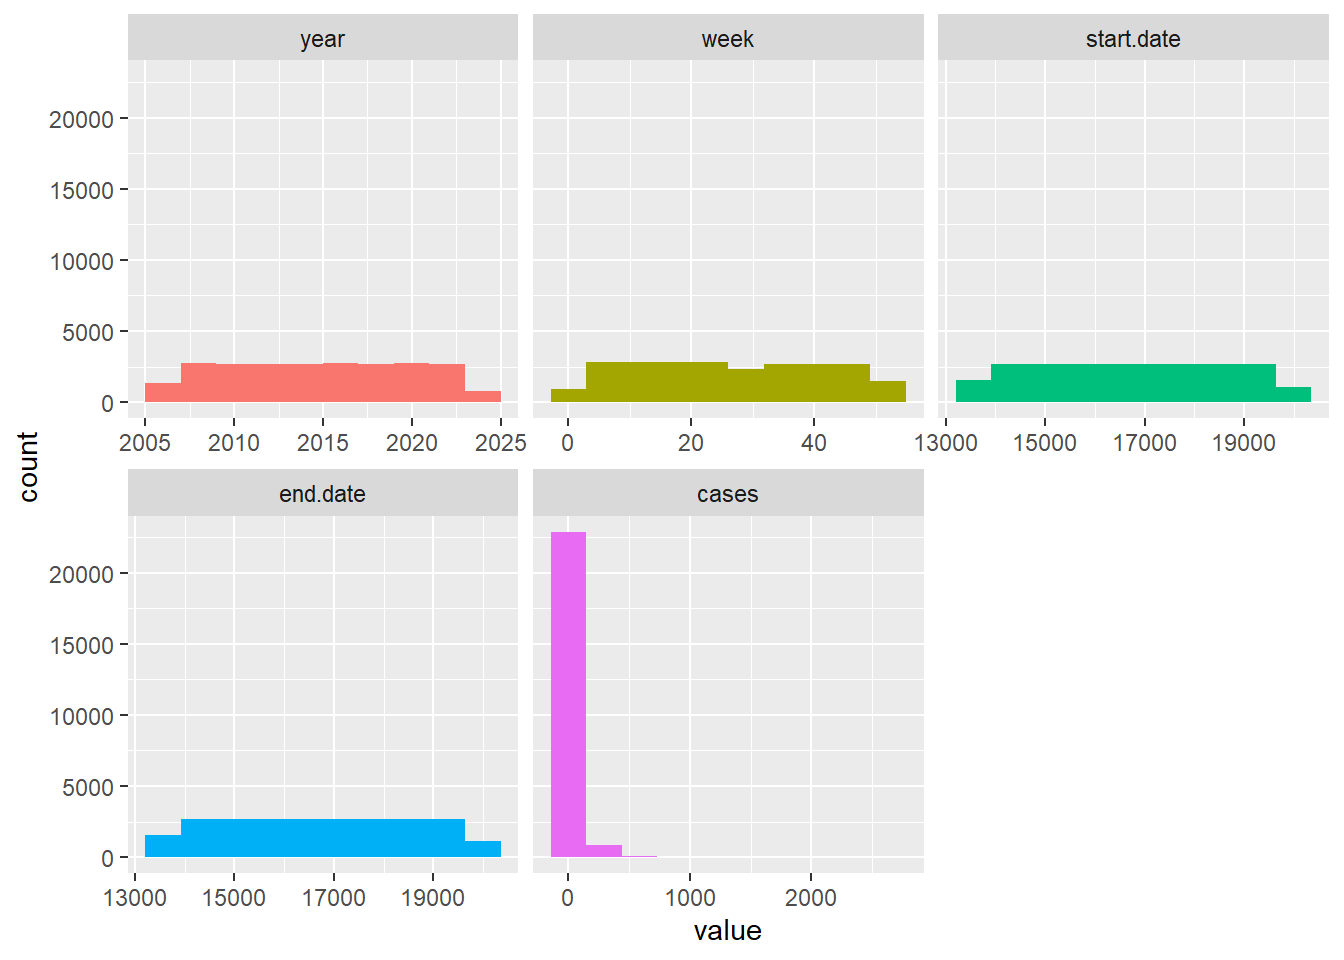
\includegraphics{ch2_files/figure-pdf/unnamed-chunk-8-1.pdf}

Distribution of Categorical Variables

R
Code:\ldots\ldots\ldots\ldots\ldots\ldots\ldots\ldots\ldots\ldots\ldots.

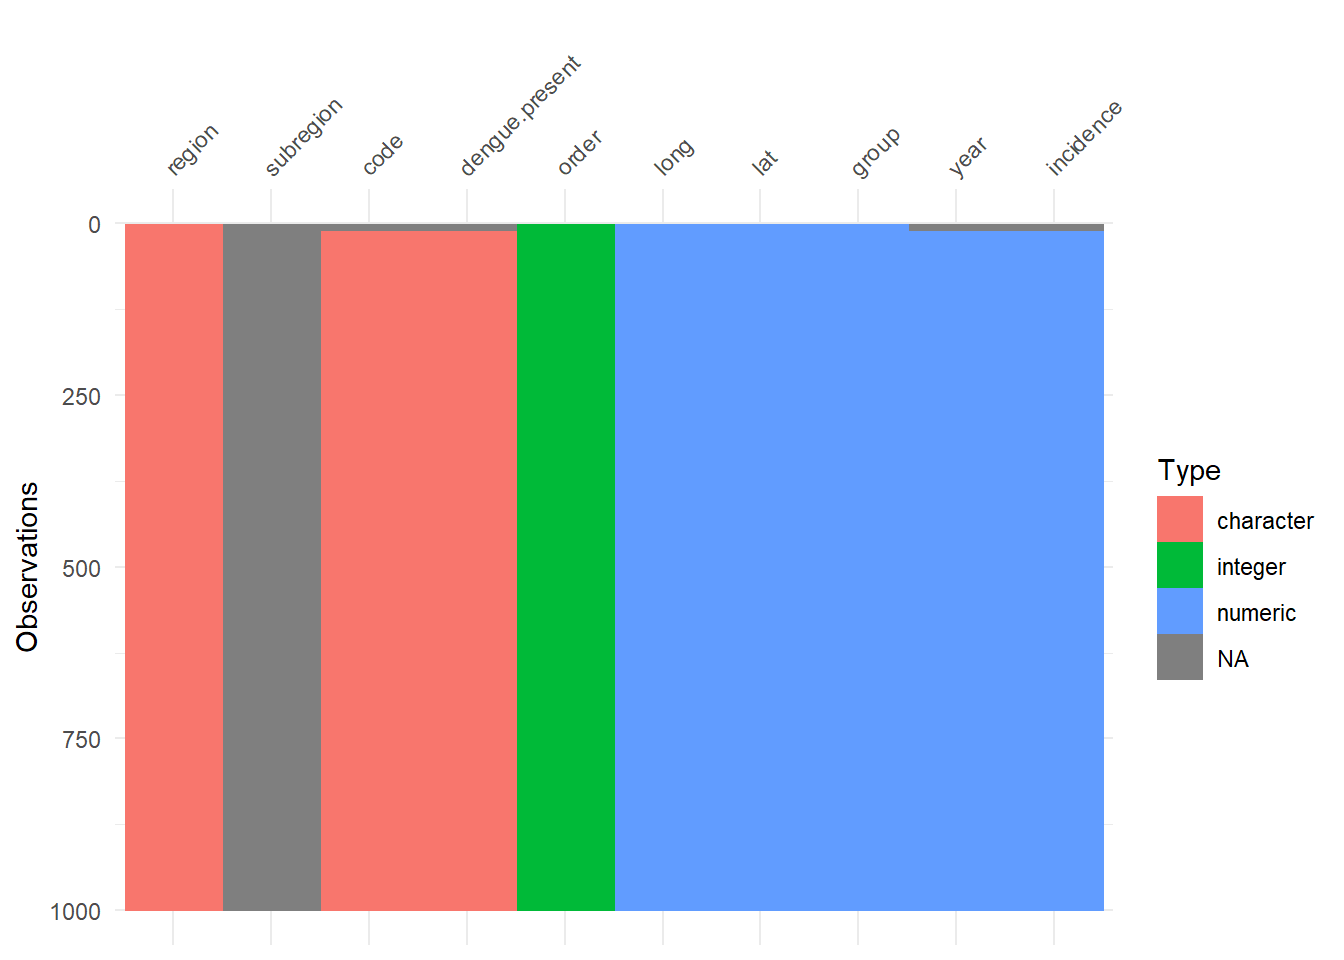
\includegraphics{ch2_files/figure-pdf/unnamed-chunk-9-1.pdf}

\begin{verbatim}
       district frequency percentage cumulative_perc
1        Ampara       920       3.85            3.85
2  Anuradhapura       920       3.85            7.70
3       Badulla       920       3.85           11.55
4    Batticaloa       920       3.85           15.40
5       Colombo       920       3.85           19.25
6         Galle       920       3.85           23.10
7       Gampaha       920       3.85           26.95
8   Hambanthota       920       3.85           30.80
9        Jaffna       920       3.85           34.65
10     Kalutara       920       3.85           38.50
11        Kandy       920       3.85           42.35
12      Kegalle       920       3.85           46.20
13  Kilinochchi       920       3.85           50.05
14   Kurunegala       920       3.85           53.90
15       Mannar       920       3.85           57.75
16       Matale       920       3.85           61.60
17       Matara       920       3.85           65.45
18   Monaragala       920       3.85           69.30
19   Mullaitivu       920       3.85           73.15
20  Polonnaruwa       920       3.85           77.00
21     Puttalam       920       3.85           80.85
22    Ratnapura       920       3.85           84.70
23  Trincomalee       920       3.85           88.55
24     Vavuniya       920       3.85           92.40
25  NuwaraEliya       911       3.81           96.21
26      Kalmune       891       3.73          100.00
\end{verbatim}

\subsubsection{Method 3}\label{method-3}

R
Code:\ldots\ldots\ldots\ldots\ldots\ldots\ldots\ldots\ldots\ldots\ldots.

\begin{verbatim}
# A tibble: 3 x 6
  variables types   missing_count missing_percent unique_count unique_rate
  <chr>     <chr>           <int>           <dbl>        <int>       <dbl>
1 year      integer             0               0            1    0.000333
2 month     integer             0               0           12    0.004   
3 day       integer             0               0           31    0.0103  
\end{verbatim}

\subsection{\texorpdfstring{Data Description:
\texttt{denguedatahub::world\_annual}}{Data Description: denguedatahub::world\_annual}}\label{data-description-denguedatahubworld_annual}

R
Code:\ldots\ldots\ldots\ldots\ldots\ldots\ldots\ldots\ldots\ldots\ldots.

\begin{longtable}[]{@{}ll@{}}
\caption{Data summary}\tabularnewline
\toprule\noalign{}
\endfirsthead
\endhead
\bottomrule\noalign{}
\endlastfoot
Name & world\_annual \\
Number of rows & 2773284 \\
Number of columns & 10 \\
\_\_\_\_\_\_\_\_\_\_\_\_\_\_\_\_\_\_\_\_\_\_\_ & \\
Column type frequency: & \\
character & 4 \\
numeric & 6 \\
\_\_\_\_\_\_\_\_\_\_\_\_\_\_\_\_\_\_\_\_\_\_\_\_ & \\
Group variables & None \\
\end{longtable}

\textbf{Variable type: character}

\begin{longtable}[]{@{}
  >{\raggedright\arraybackslash}p{(\columnwidth - 14\tabcolsep) * \real{0.2055}}
  >{\raggedleft\arraybackslash}p{(\columnwidth - 14\tabcolsep) * \real{0.1370}}
  >{\raggedleft\arraybackslash}p{(\columnwidth - 14\tabcolsep) * \real{0.1918}}
  >{\raggedleft\arraybackslash}p{(\columnwidth - 14\tabcolsep) * \real{0.0548}}
  >{\raggedleft\arraybackslash}p{(\columnwidth - 14\tabcolsep) * \real{0.0548}}
  >{\raggedleft\arraybackslash}p{(\columnwidth - 14\tabcolsep) * \real{0.0822}}
  >{\raggedleft\arraybackslash}p{(\columnwidth - 14\tabcolsep) * \real{0.1233}}
  >{\raggedleft\arraybackslash}p{(\columnwidth - 14\tabcolsep) * \real{0.1507}}@{}}
\toprule\noalign{}
\begin{minipage}[b]{\linewidth}\raggedright
skim\_variable
\end{minipage} & \begin{minipage}[b]{\linewidth}\raggedleft
n\_missing
\end{minipage} & \begin{minipage}[b]{\linewidth}\raggedleft
complete\_rate
\end{minipage} & \begin{minipage}[b]{\linewidth}\raggedleft
min
\end{minipage} & \begin{minipage}[b]{\linewidth}\raggedleft
max
\end{minipage} & \begin{minipage}[b]{\linewidth}\raggedleft
empty
\end{minipage} & \begin{minipage}[b]{\linewidth}\raggedleft
n\_unique
\end{minipage} & \begin{minipage}[b]{\linewidth}\raggedleft
whitespace
\end{minipage} \\
\midrule\noalign{}
\endhead
\bottomrule\noalign{}
\endlastfoot
region & 0 & 1.00 & 2 & 35 & 0 & 282 & 0 \\
subregion & 1783783 & 0.36 & 1 & 33 & 0 & 1069 & 0 \\
code & 7854 & 1.00 & 3 & 8 & 0 & 202 & 0 \\
dengue.present & 7164 & 1.00 & 2 & 3 & 0 & 2 & 0 \\
\end{longtable}

\textbf{Variable type: numeric}

\begin{longtable}[]{@{}
  >{\raggedright\arraybackslash}p{(\columnwidth - 20\tabcolsep) * \real{0.1250}}
  >{\raggedleft\arraybackslash}p{(\columnwidth - 20\tabcolsep) * \real{0.0893}}
  >{\raggedleft\arraybackslash}p{(\columnwidth - 20\tabcolsep) * \real{0.1250}}
  >{\raggedleft\arraybackslash}p{(\columnwidth - 20\tabcolsep) * \real{0.0893}}
  >{\raggedleft\arraybackslash}p{(\columnwidth - 20\tabcolsep) * \real{0.0982}}
  >{\raggedleft\arraybackslash}p{(\columnwidth - 20\tabcolsep) * \real{0.0714}}
  >{\raggedleft\arraybackslash}p{(\columnwidth - 20\tabcolsep) * \real{0.0804}}
  >{\raggedleft\arraybackslash}p{(\columnwidth - 20\tabcolsep) * \real{0.0804}}
  >{\raggedleft\arraybackslash}p{(\columnwidth - 20\tabcolsep) * \real{0.0804}}
  >{\raggedleft\arraybackslash}p{(\columnwidth - 20\tabcolsep) * \real{0.1071}}
  >{\raggedright\arraybackslash}p{(\columnwidth - 20\tabcolsep) * \real{0.0536}}@{}}
\toprule\noalign{}
\begin{minipage}[b]{\linewidth}\raggedright
skim\_variable
\end{minipage} & \begin{minipage}[b]{\linewidth}\raggedleft
n\_missing
\end{minipage} & \begin{minipage}[b]{\linewidth}\raggedleft
complete\_rate
\end{minipage} & \begin{minipage}[b]{\linewidth}\raggedleft
mean
\end{minipage} & \begin{minipage}[b]{\linewidth}\raggedleft
sd
\end{minipage} & \begin{minipage}[b]{\linewidth}\raggedleft
p0
\end{minipage} & \begin{minipage}[b]{\linewidth}\raggedleft
p25
\end{minipage} & \begin{minipage}[b]{\linewidth}\raggedleft
p50
\end{minipage} & \begin{minipage}[b]{\linewidth}\raggedleft
p75
\end{minipage} & \begin{minipage}[b]{\linewidth}\raggedleft
p100
\end{minipage} & \begin{minipage}[b]{\linewidth}\raggedright
hist
\end{minipage} \\
\midrule\noalign{}
\endhead
\bottomrule\noalign{}
\endlastfoot
long & 900 & 1 & 12.64 & 85.44 & -180.00 & -67.60 & 19.10 & 80.68 &
190.27 & ▂▆▇▆▃ \\
lat & 900 & 1 & 30.24 & 32.65 & -85.19 & 6.95 & 36.81 & 55.33 & 83.60 &
▁▂▆▇▇ \\
group & 900 & 1 & 834.10 & 457.79 & 1.00 & 417.00 & 847.00 & 1296.00 &
1627.00 & ▅▇▆▅▇ \\
order & 900 & 1 & 52582.05 & 28142.60 & 1.00 & 28173.00 & 52658.00 &
77045.00 & 100964.00 & ▆▇▇▇▇ \\
year & 7164 & 1 & 2004.50 & 8.66 & 1990.00 & 1997.00 & 2004.50 & 2012.00
& 2019.00 & ▇▇▇▇▇ \\
incidence & 7164 & 1 & 701055.46 & 3036888.47 & 0.00 & 0.00 & 0.00 &
99597.00 & 56878730.00 & ▇▁▁▁▁ \\
\end{longtable}

Method 2:

\begin{Shaded}
\begin{Highlighting}[]
\FunctionTok{status}\NormalTok{(world\_annual)}
\end{Highlighting}
\end{Shaded}

\begin{verbatim}
                     variable q_zeros      p_zeros    q_na        p_na q_inf
long                     long     721 0.0002599806     900 0.000324525     0
lat                       lat       0 0.0000000000     900 0.000324525     0
group                   group       0 0.0000000000     900 0.000324525     0
order                   order       0 0.0000000000     900 0.000324525     0
region                 region       0 0.0000000000       0 0.000000000     0
subregion           subregion       0 0.0000000000 1783783 0.643202427     0
code                     code       0 0.0000000000    7854 0.002832022     0
year                     year       0 0.0000000000    7164 0.002583219     0
incidence           incidence 1423590 0.5133228331    7164 0.002583219     0
dengue.present dengue.present       0 0.0000000000    7164 0.002583219     0
               p_inf      type unique
long               0   numeric  76880
lat                0   numeric  76361
group              0   numeric   1627
order              0   integer  99338
region             0 character    282
subregion          0 character   1069
code               0 character    202
year               0   numeric     30
incidence          0   numeric   4109
dengue.present     0 character      2
\end{verbatim}

\begin{Shaded}
\begin{Highlighting}[]
\FunctionTok{data\_integrity}\NormalTok{(world\_annual)}
\end{Highlighting}
\end{Shaded}

\begin{verbatim}
$vars_num_with_NA
           variable q_na        p_na
long           long  900 0.000324525
lat             lat  900 0.000324525
group         group  900 0.000324525
order         order  900 0.000324525
year           year 7164 0.002583219
incidence incidence 7164 0.002583219

$vars_cat_with_NA
                     variable    q_na        p_na
subregion           subregion 1783783 0.643202427
code                     code    7854 0.002832022
dengue.present dengue.present    7164 0.002583219

$vars_cat_high_card
           variable unique
subregion subregion   1069
region       region    282
code           code    202

$MAX_UNIQUE
[1] 35

$vars_one_value
character(0)

$vars_cat
[1] "region"         "subregion"      "code"           "dengue.present"

$vars_num
[1] "long"      "lat"       "group"     "order"     "year"      "incidence"

$vars_char
[1] "region"         "subregion"      "code"           "dengue.present"

$vars_factor
character(0)

$vars_other
character(0)
\end{verbatim}

\begin{Shaded}
\begin{Highlighting}[]
\FunctionTok{profiling\_num}\NormalTok{(world\_annual)}
\end{Highlighting}
\end{Shaded}

\begin{verbatim}
   variable         mean      std_dev variation_coef      p_01       p_05
1      long     12.63966 8.543838e+01    6.759545411 -164.0733 -125.18413
2       lat     30.24176 3.265450e+01    1.079781713  -51.7249  -29.59932
3     group    834.10077 4.577919e+02    0.548844831   10.0000  184.00000
4     order  52582.04712 2.814260e+04    0.535213158  949.0000 9447.00000
5      year   2004.50000 8.655443e+00    0.004318006 1990.0000 1991.00000
6 incidence 701055.45849 3.036888e+06    4.331880495    0.0000    0.00000
          p_25        p_50        p_75         p_95         p_99    skewness
1   -67.596336    19.09844    80.68213 1.445178e+02 1.746725e+02 -0.07340286
2     6.946973    36.81196    55.33027 7.582597e+01 8.078438e+01 -0.51056358
3   417.000000   847.00000  1296.00000 1.569000e+03 1.621000e+03  0.06183424
4 28173.000000 52658.00000 77045.00000 9.621100e+04 1.000290e+05 -0.02092148
5  1997.000000  2004.50000  2012.00000 2.018000e+03 2.019000e+03  0.00000000
6     0.000000     0.00000 99597.00000 2.616088e+06 2.137839e+07  7.04612715
   kurtosis        iqr                              range_98
1  2.091961   148.2785 [-164.073287963867, 174.672546386719]
2  2.553684    48.3833 [-51.7249031066895, 80.7843780517578]
3  1.727049   879.0000                            [10, 1621]
4  1.826357 48872.0000                         [949, 100029]
5  1.797330    15.0000                          [1990, 2019]
6 55.475409 99597.0000                         [0, 21378391]
                              range_80
1 [-95.987060546875, 126.757331848145]
2  [-14.16845703125, 70.2992172241211]
3                          [242, 1441]
4                       [14136, 91463]
5 [1992.90000000002, 2016.10000000009]
6                         [0, 1723528]
\end{verbatim}

Distribution of Numeric Variables

\begin{Shaded}
\begin{Highlighting}[]
\FunctionTok{plot\_num}\NormalTok{(world\_annual)}
\end{Highlighting}
\end{Shaded}

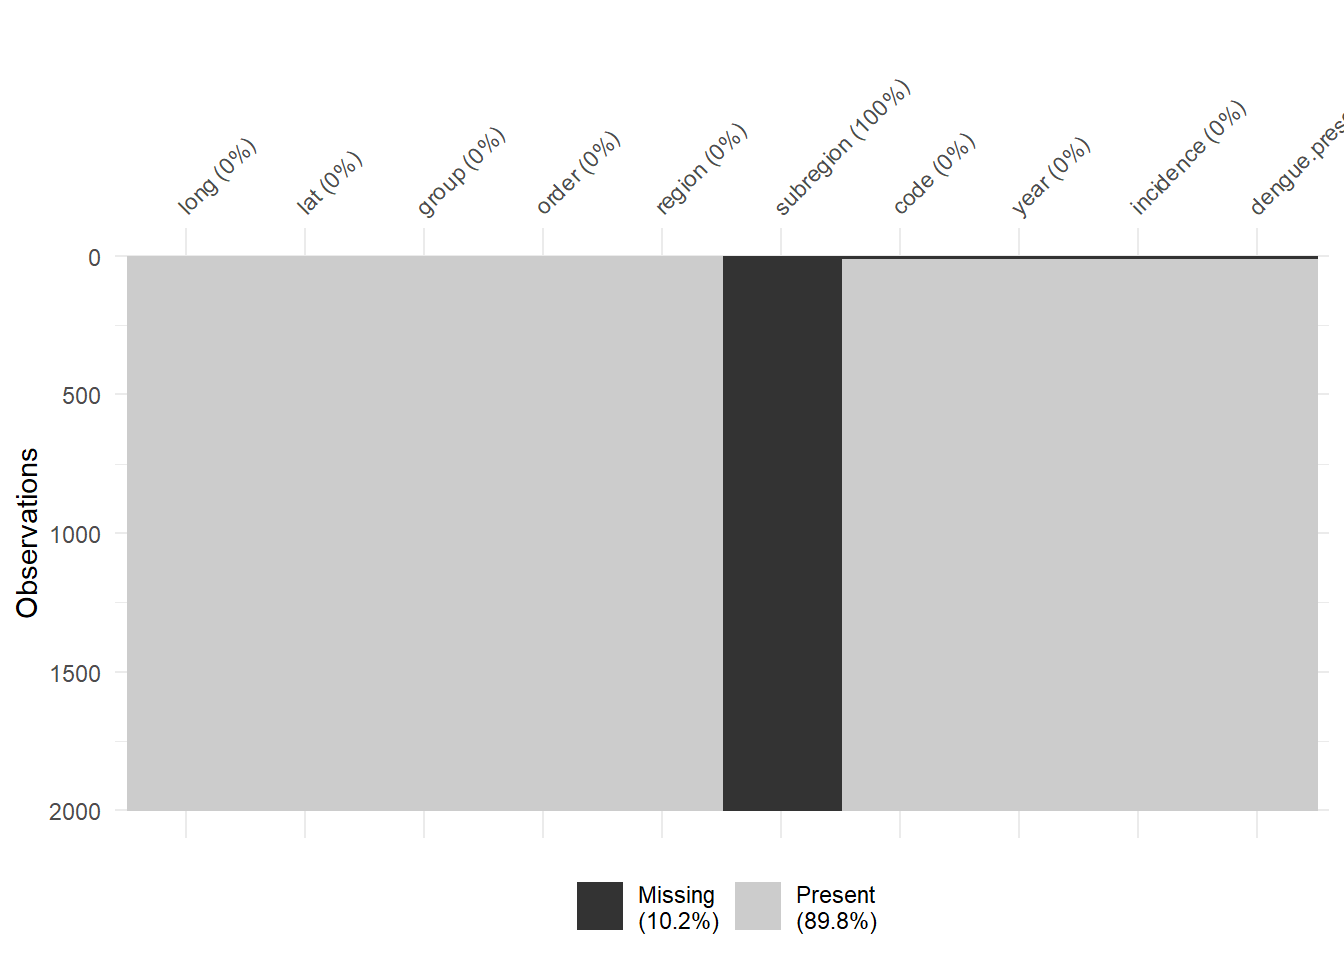
\includegraphics{ch2_files/figure-pdf/unnamed-chunk-15-1.pdf}

Distribution of Categorical Variables

\begin{Shaded}
\begin{Highlighting}[]
\FunctionTok{freq}\NormalTok{(world\_annual)}
\end{Highlighting}
\end{Shaded}

Note: Output has been omitted due to its length.

\section{Variable Types}\label{variable-types}

\subsection{\texorpdfstring{\texttt{denguedatahub::srilanka\_weekly\_data}}{denguedatahub::srilanka\_weekly\_data}}\label{denguedatahubsrilanka_weekly_data}

R
Code:\ldots\ldots\ldots\ldots\ldots\ldots\ldots\ldots\ldots\ldots\ldots.

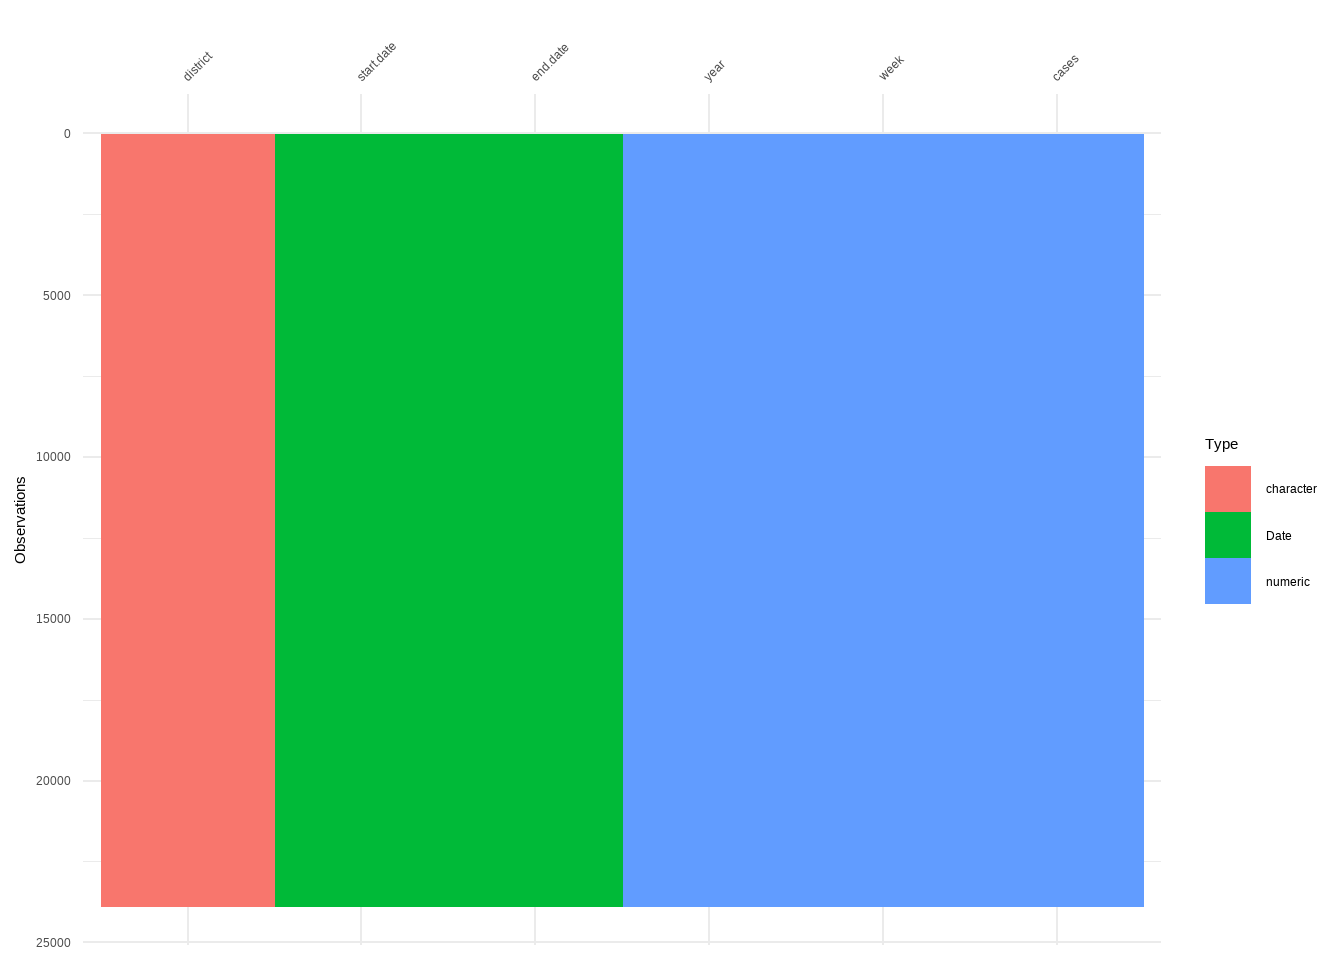
\includegraphics{ch2_files/figure-pdf/unnamed-chunk-17-1.pdf}

Question: Why is there no observable variability in the \texttt{cases}
column?

\subsection{\texorpdfstring{\texttt{denguedatahub::world\_annual}}{denguedatahub::world\_annual}}\label{denguedatahubworld_annual}

This example shows how to work with a large dataset with \texttt{visdat}

R
Code:\ldots\ldots\ldots\ldots\ldots\ldots\ldots\ldots\ldots\ldots\ldots.

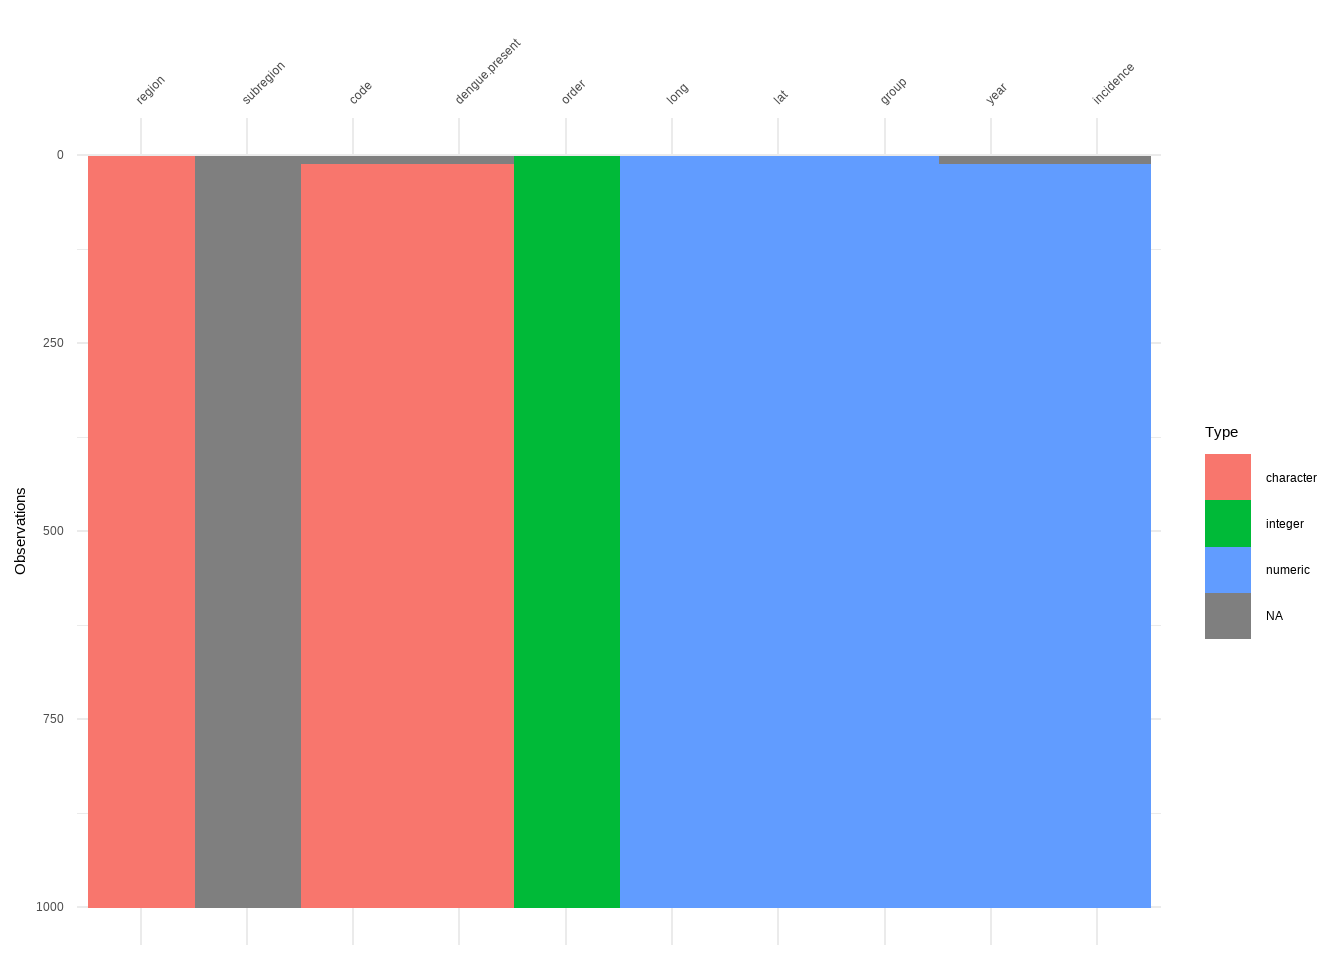
\includegraphics{ch2_files/figure-pdf/unnamed-chunk-18-1.pdf}

\section{Visualising Numerial Data}\label{visualising-numerial-data}

\subsection{\texorpdfstring{\texttt{denguedatahub::srilanka\_weekly\_data}}{denguedatahub::srilanka\_weekly\_data}}\label{denguedatahubsrilanka_weekly_data-1}

R
Code:\ldots\ldots\ldots\ldots\ldots\ldots\ldots\ldots\ldots\ldots\ldots.

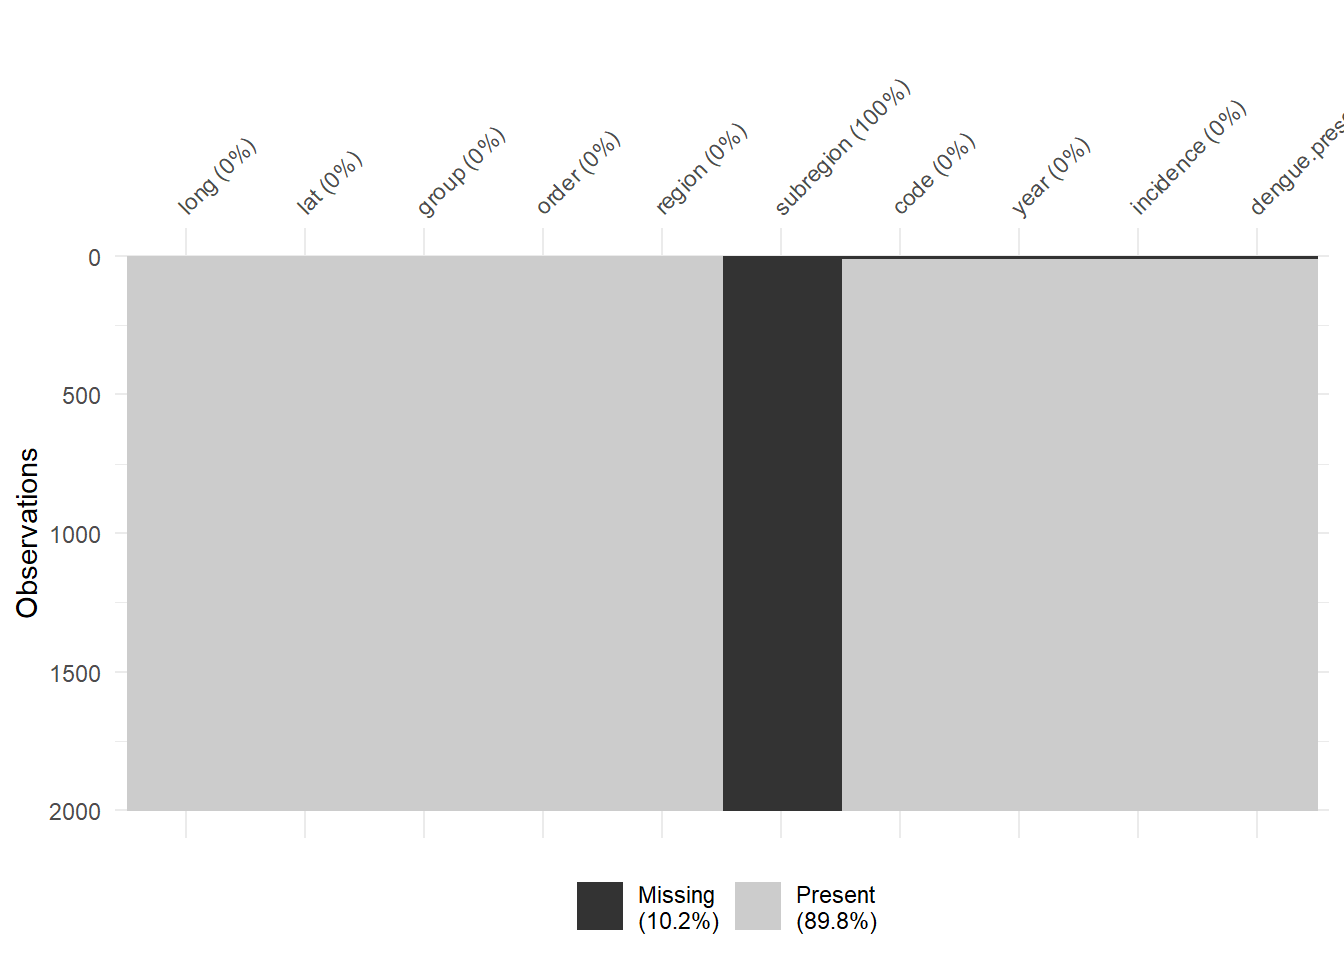
\includegraphics{ch2_files/figure-pdf/unnamed-chunk-19-1.pdf}

\subsection{\texorpdfstring{\texttt{denguedatahub::world\_annual}}{denguedatahub::world\_annual}}\label{denguedatahubworld_annual-1}

R
Code:\ldots\ldots\ldots\ldots\ldots\ldots\ldots\ldots\ldots\ldots\ldots.

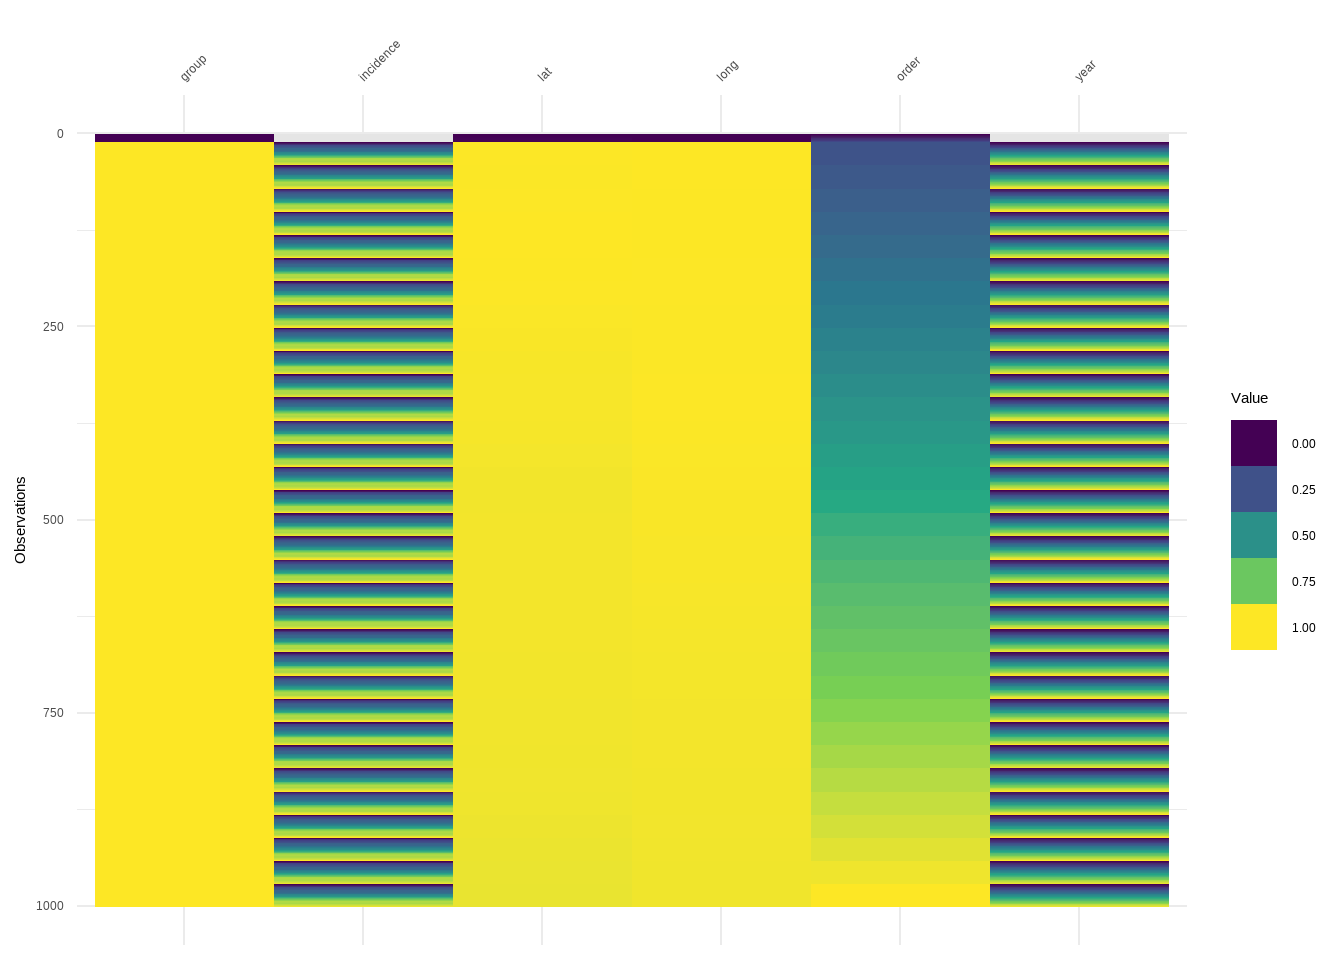
\includegraphics{ch2_files/figure-pdf/unnamed-chunk-20-1.pdf}

\section{Arrange Data Before Plotting Numeric
Variables}\label{arrange-data-before-plotting-numeric-variables}

\subsection{\texorpdfstring{\texttt{denguedatahub::srilanka\_weekly\_data}}{denguedatahub::srilanka\_weekly\_data}}\label{denguedatahubsrilanka_weekly_data-2}

R
Code:\ldots\ldots\ldots\ldots\ldots\ldots\ldots\ldots\ldots\ldots\ldots.

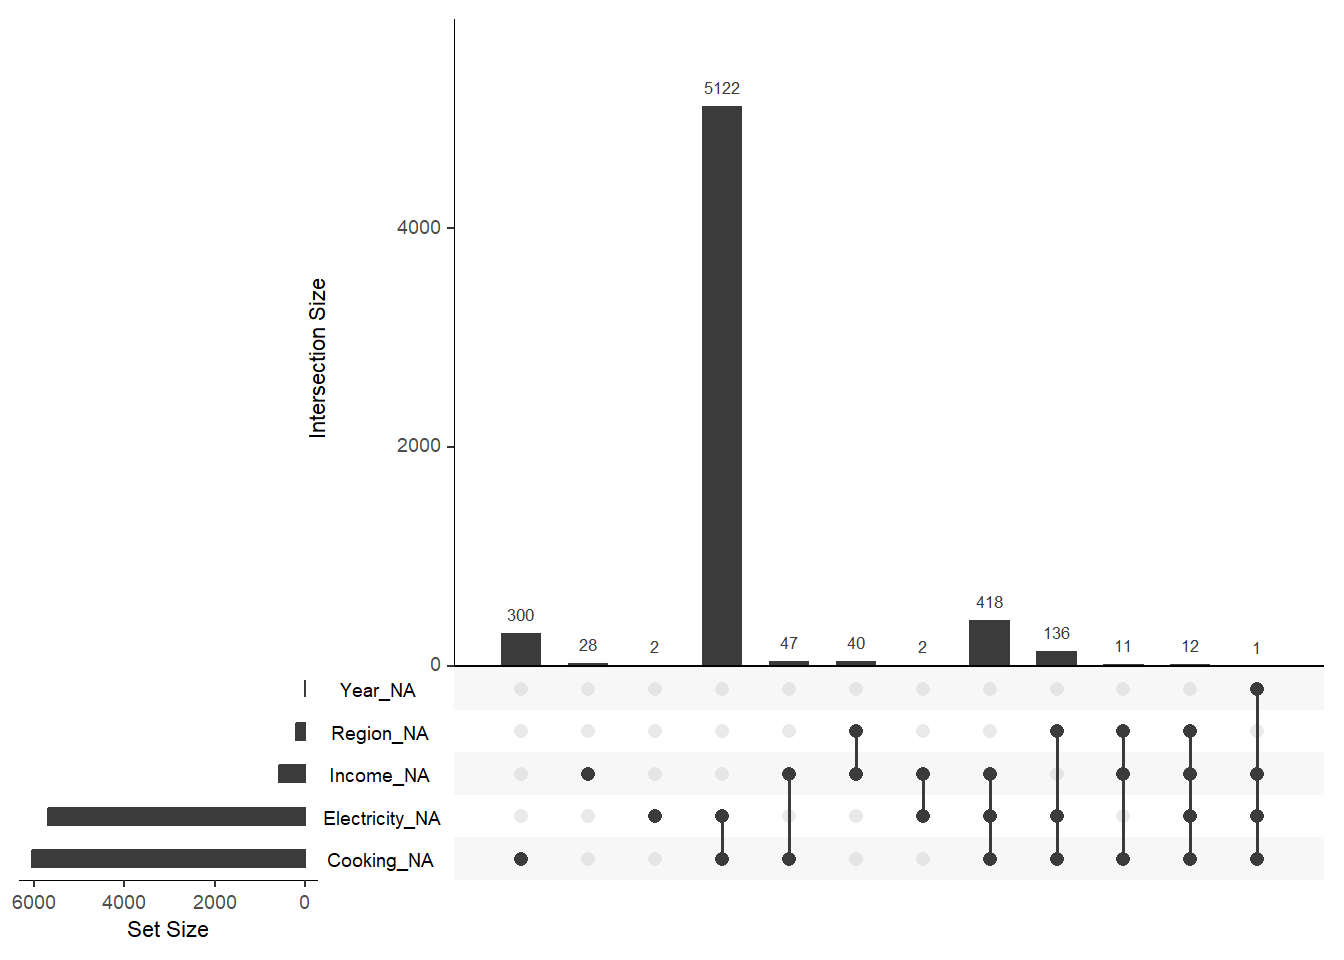
\includegraphics{ch2_files/figure-pdf/unnamed-chunk-21-1.pdf}

\section{Visualise Binary Variables in the
Data}\label{visualise-binary-variables-in-the-data}

\begin{Shaded}
\begin{Highlighting}[]
\DocumentationTok{\#\# Sample dataset}
\NormalTok{df1 }\OtherTok{\textless{}{-}} \FunctionTok{tibble}\NormalTok{(}\AttributeTok{x=}\FunctionTok{rep}\NormalTok{(}\FunctionTok{c}\NormalTok{(}\DecValTok{1}\NormalTok{, }\DecValTok{0}\NormalTok{), }\DecValTok{50}\NormalTok{), }\AttributeTok{y=}\FunctionTok{c}\NormalTok{(}\FunctionTok{rep}\NormalTok{(}\DecValTok{1}\NormalTok{, }\DecValTok{50}\NormalTok{), }\FunctionTok{rep}\NormalTok{(}\DecValTok{0}\NormalTok{, }\DecValTok{50}\NormalTok{)))}
\end{Highlighting}
\end{Shaded}

R
Code:\ldots\ldots\ldots\ldots\ldots\ldots\ldots\ldots\ldots\ldots\ldots.

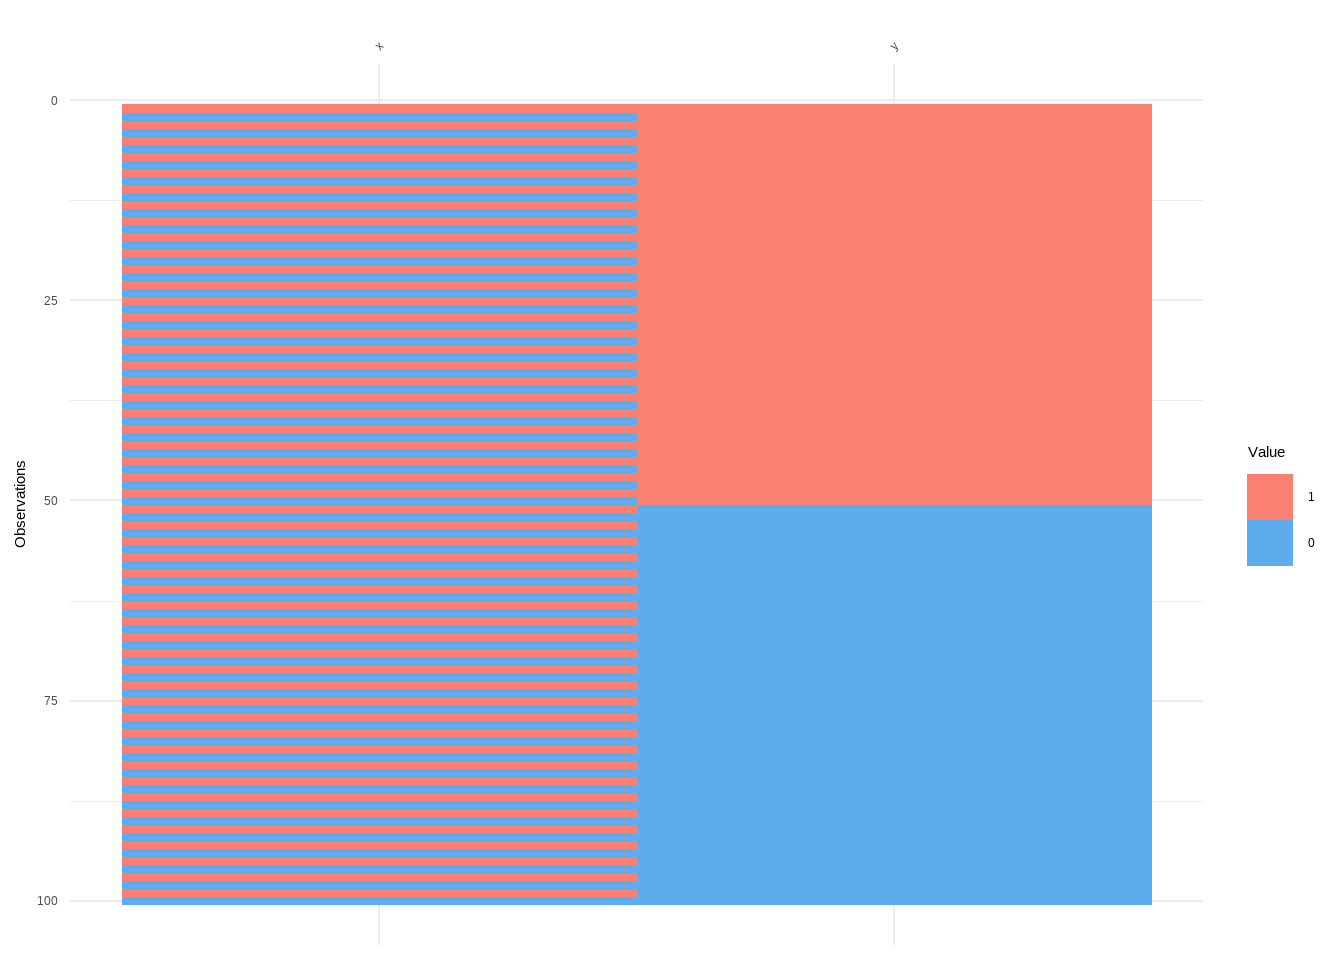
\includegraphics{ch2_files/figure-pdf/unnamed-chunk-23-1.pdf}

\section{Visualise Messy Data Sets with Mixed Data
Types}\label{visualise-messy-data-sets-with-mixed-data-types}

R
Code:\ldots\ldots\ldots\ldots\ldots\ldots\ldots\ldots\ldots\ldots\ldots.

\begin{verbatim}
# A tibble: 10 x 3
   x        y        z       
   <chr>    <chr>    <chr>   
 1 TRUE     200      30.5    
 2 TRUE     30.5     TRUE    
 3 1        TRUE     TRUE    
 4 200      0        1       
 5 1        2014/1/2 1       
 6 30       1        0       
 7 30.5     1        1       
 8 1        1        30      
 9 0        TRUE     200     
10 2014/1/2 30       2014/1/2
\end{verbatim}

\subsection{Visualise the Data Set}\label{visualise-the-data-set}

R
Code:\ldots\ldots\ldots\ldots\ldots\ldots\ldots\ldots\ldots\ldots\ldots.

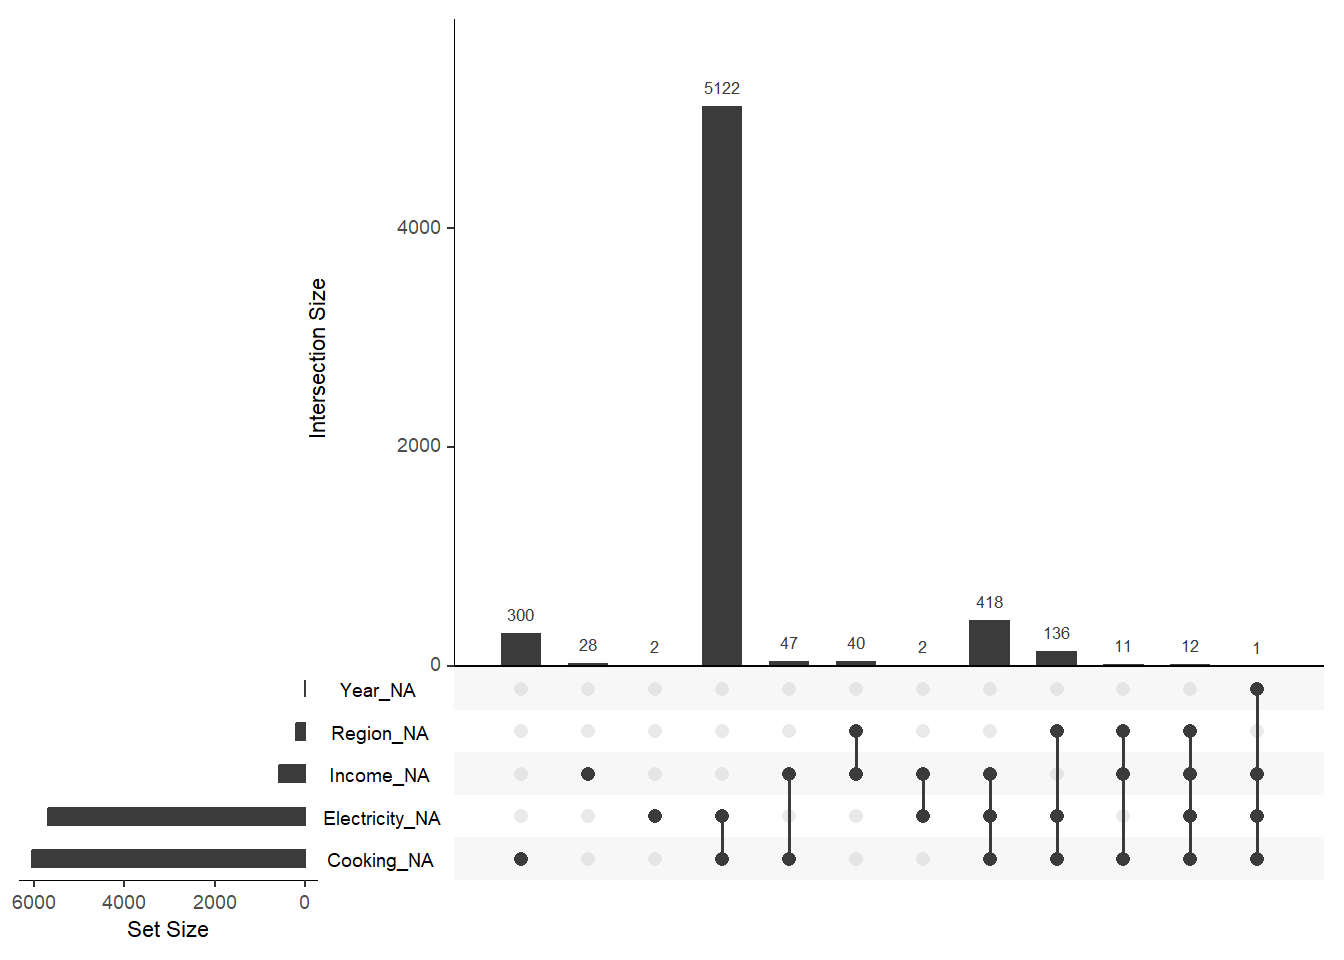
\includegraphics{ch2_files/figure-pdf/unnamed-chunk-25-1.pdf}

\subsection{Cell Identification Challenge: Guess the Function of Each
Cell}\label{cell-identification-challenge-guess-the-function-of-each-cell}

\begin{Shaded}
\begin{Highlighting}[]
\FunctionTok{vis\_guess}\NormalTok{(df2)}
\end{Highlighting}
\end{Shaded}

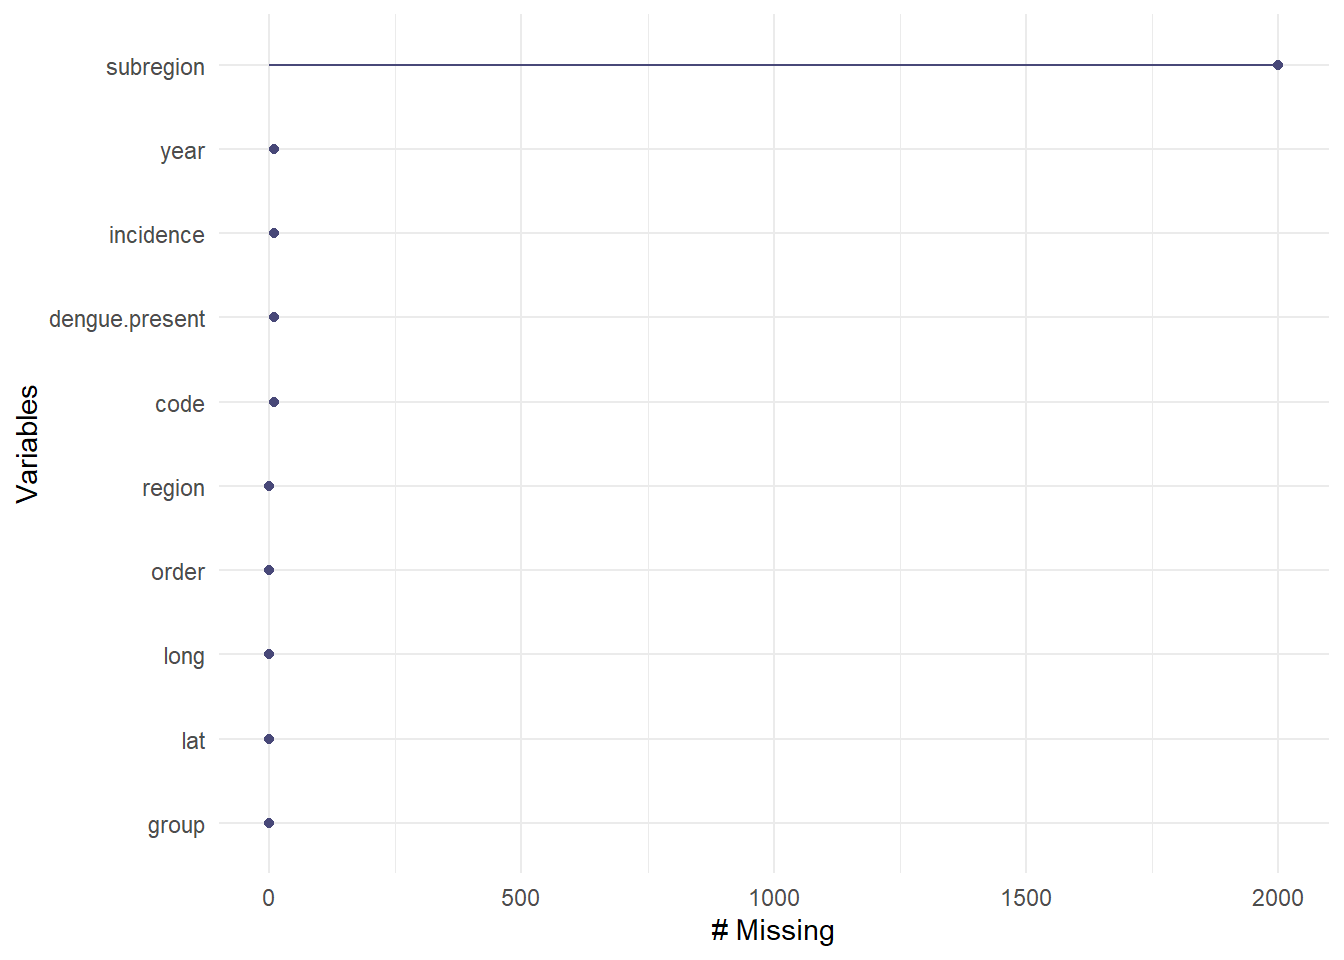
\includegraphics{ch2_files/figure-pdf/unnamed-chunk-26-1.pdf}

\section{Data Completeness}\label{data-completeness}

\subsection{Visualize the distribution of missing
data.}\label{visualize-the-distribution-of-missing-data.}

\subsubsection{\texorpdfstring{\texttt{denguedatahub::srilanka\_weekly\_data}}{denguedatahub::srilanka\_weekly\_data}}\label{denguedatahubsrilanka_weekly_data-3}

R
Code:\ldots\ldots\ldots\ldots\ldots\ldots\ldots\ldots\ldots\ldots\ldots.

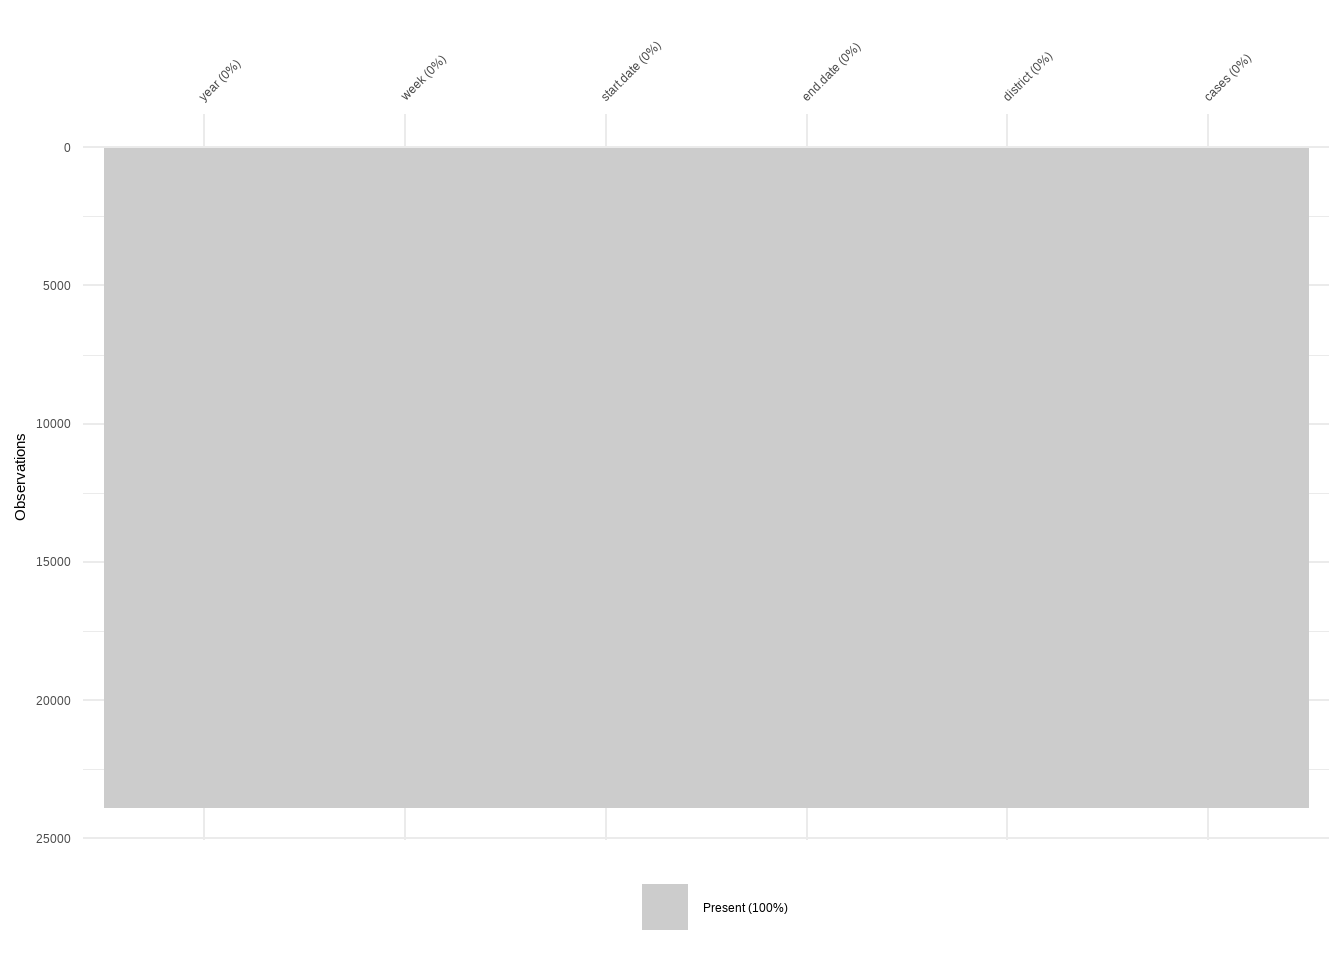
\includegraphics{ch2_files/figure-pdf/unnamed-chunk-27-1.pdf}

\subsubsection{\texorpdfstring{\texttt{denguedatahub::world\_annual}}{denguedatahub::world\_annual}}\label{denguedatahubworld_annual-2}

R
Code:\ldots\ldots\ldots\ldots\ldots\ldots\ldots\ldots\ldots\ldots\ldots.

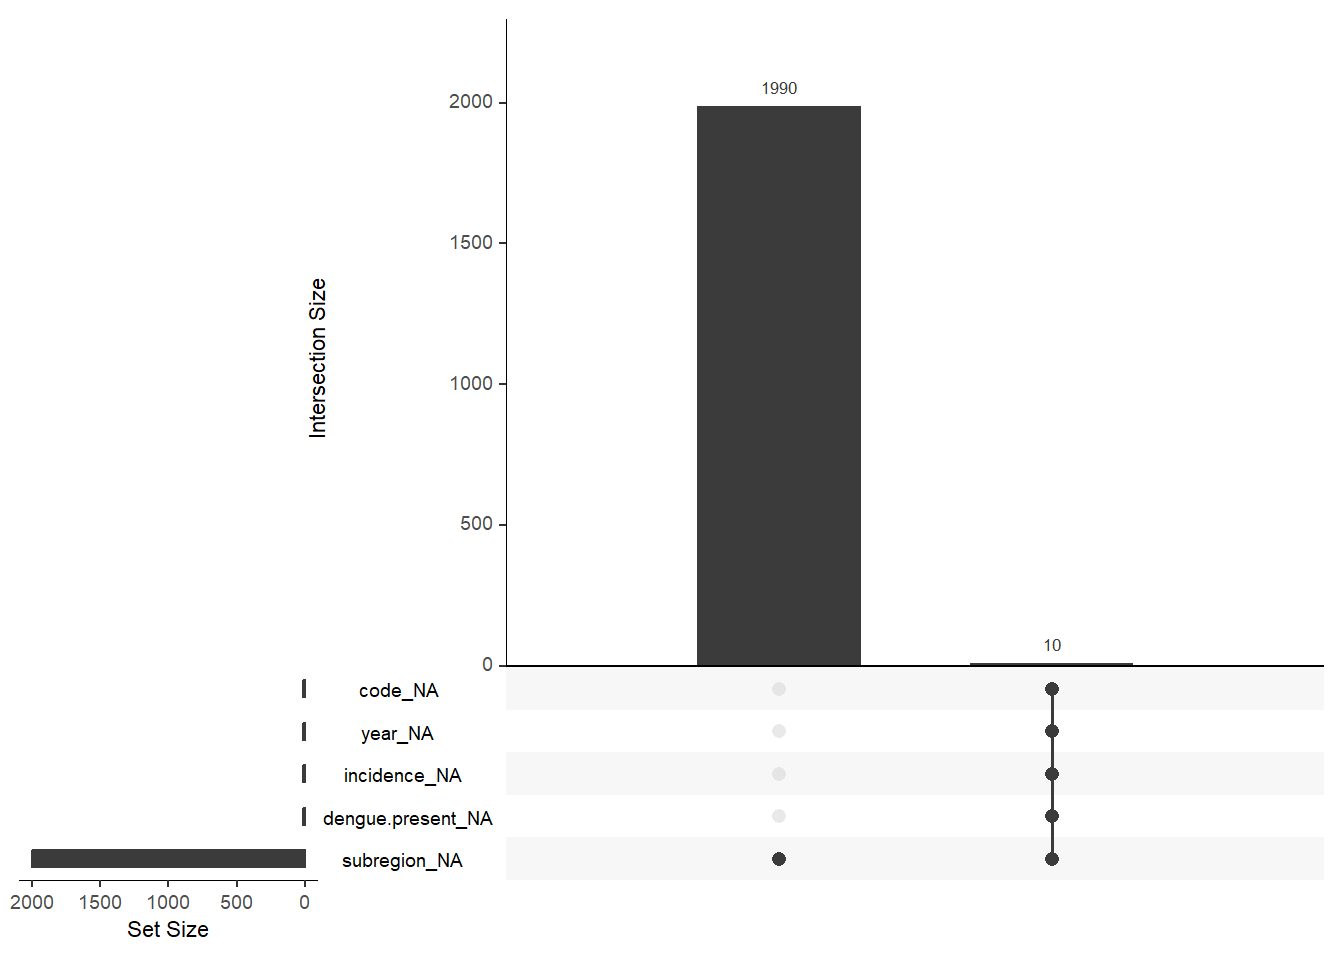
\includegraphics{ch2_files/figure-pdf/unnamed-chunk-28-1.pdf}

\subsection{Visualise Missing in
Variables}\label{visualise-missing-in-variables}

R
Code:\ldots\ldots\ldots\ldots\ldots\ldots\ldots\ldots\ldots\ldots\ldots.

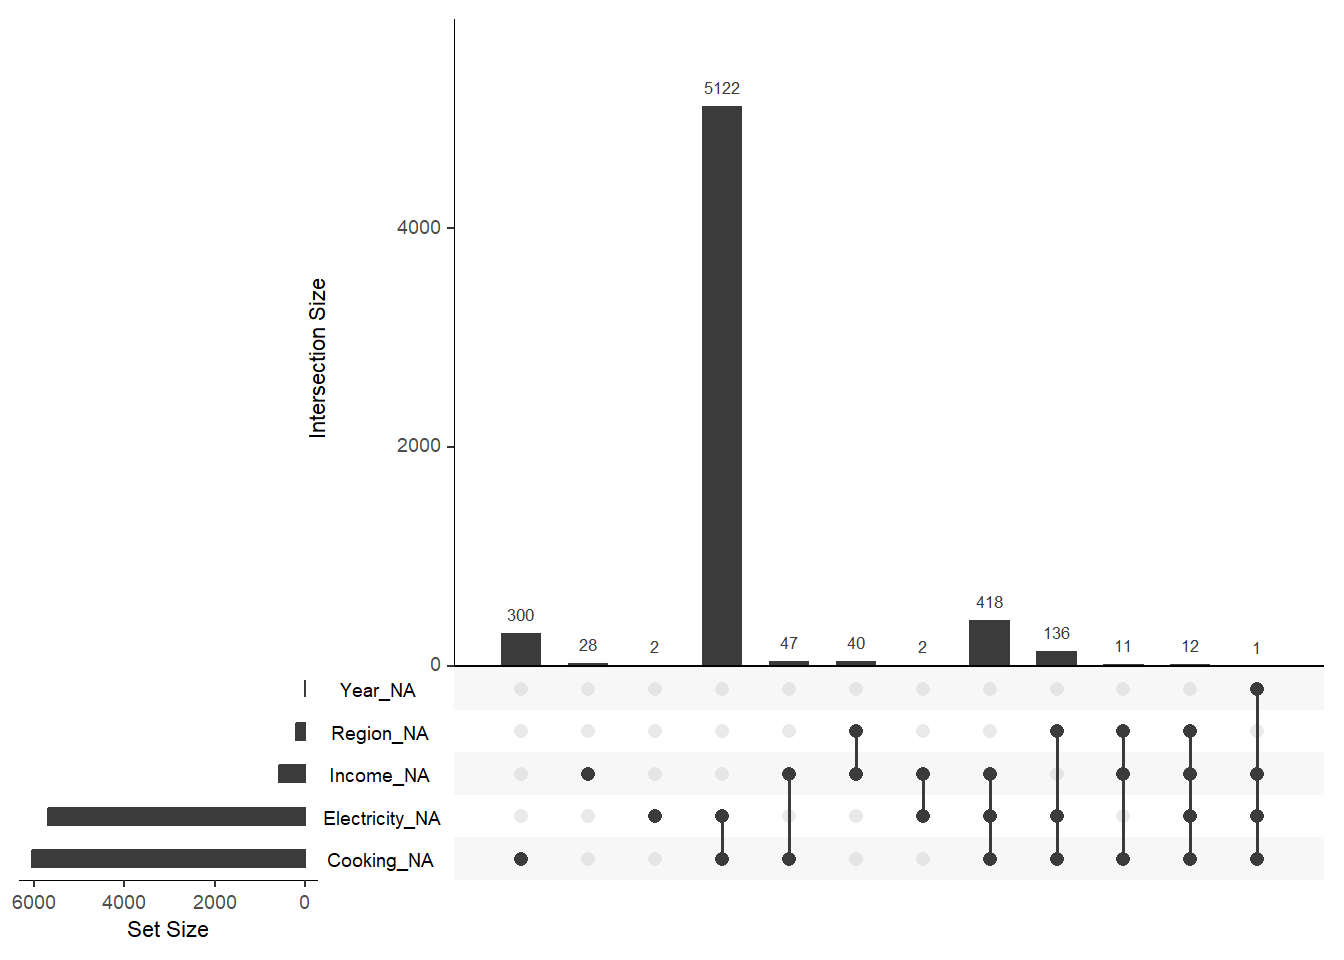
\includegraphics{ch2_files/figure-pdf/unnamed-chunk-29-1.pdf}

Small multiples of the same plot facet by year

R
Code:\ldots\ldots\ldots\ldots\ldots\ldots\ldots\ldots\ldots\ldots\ldots.

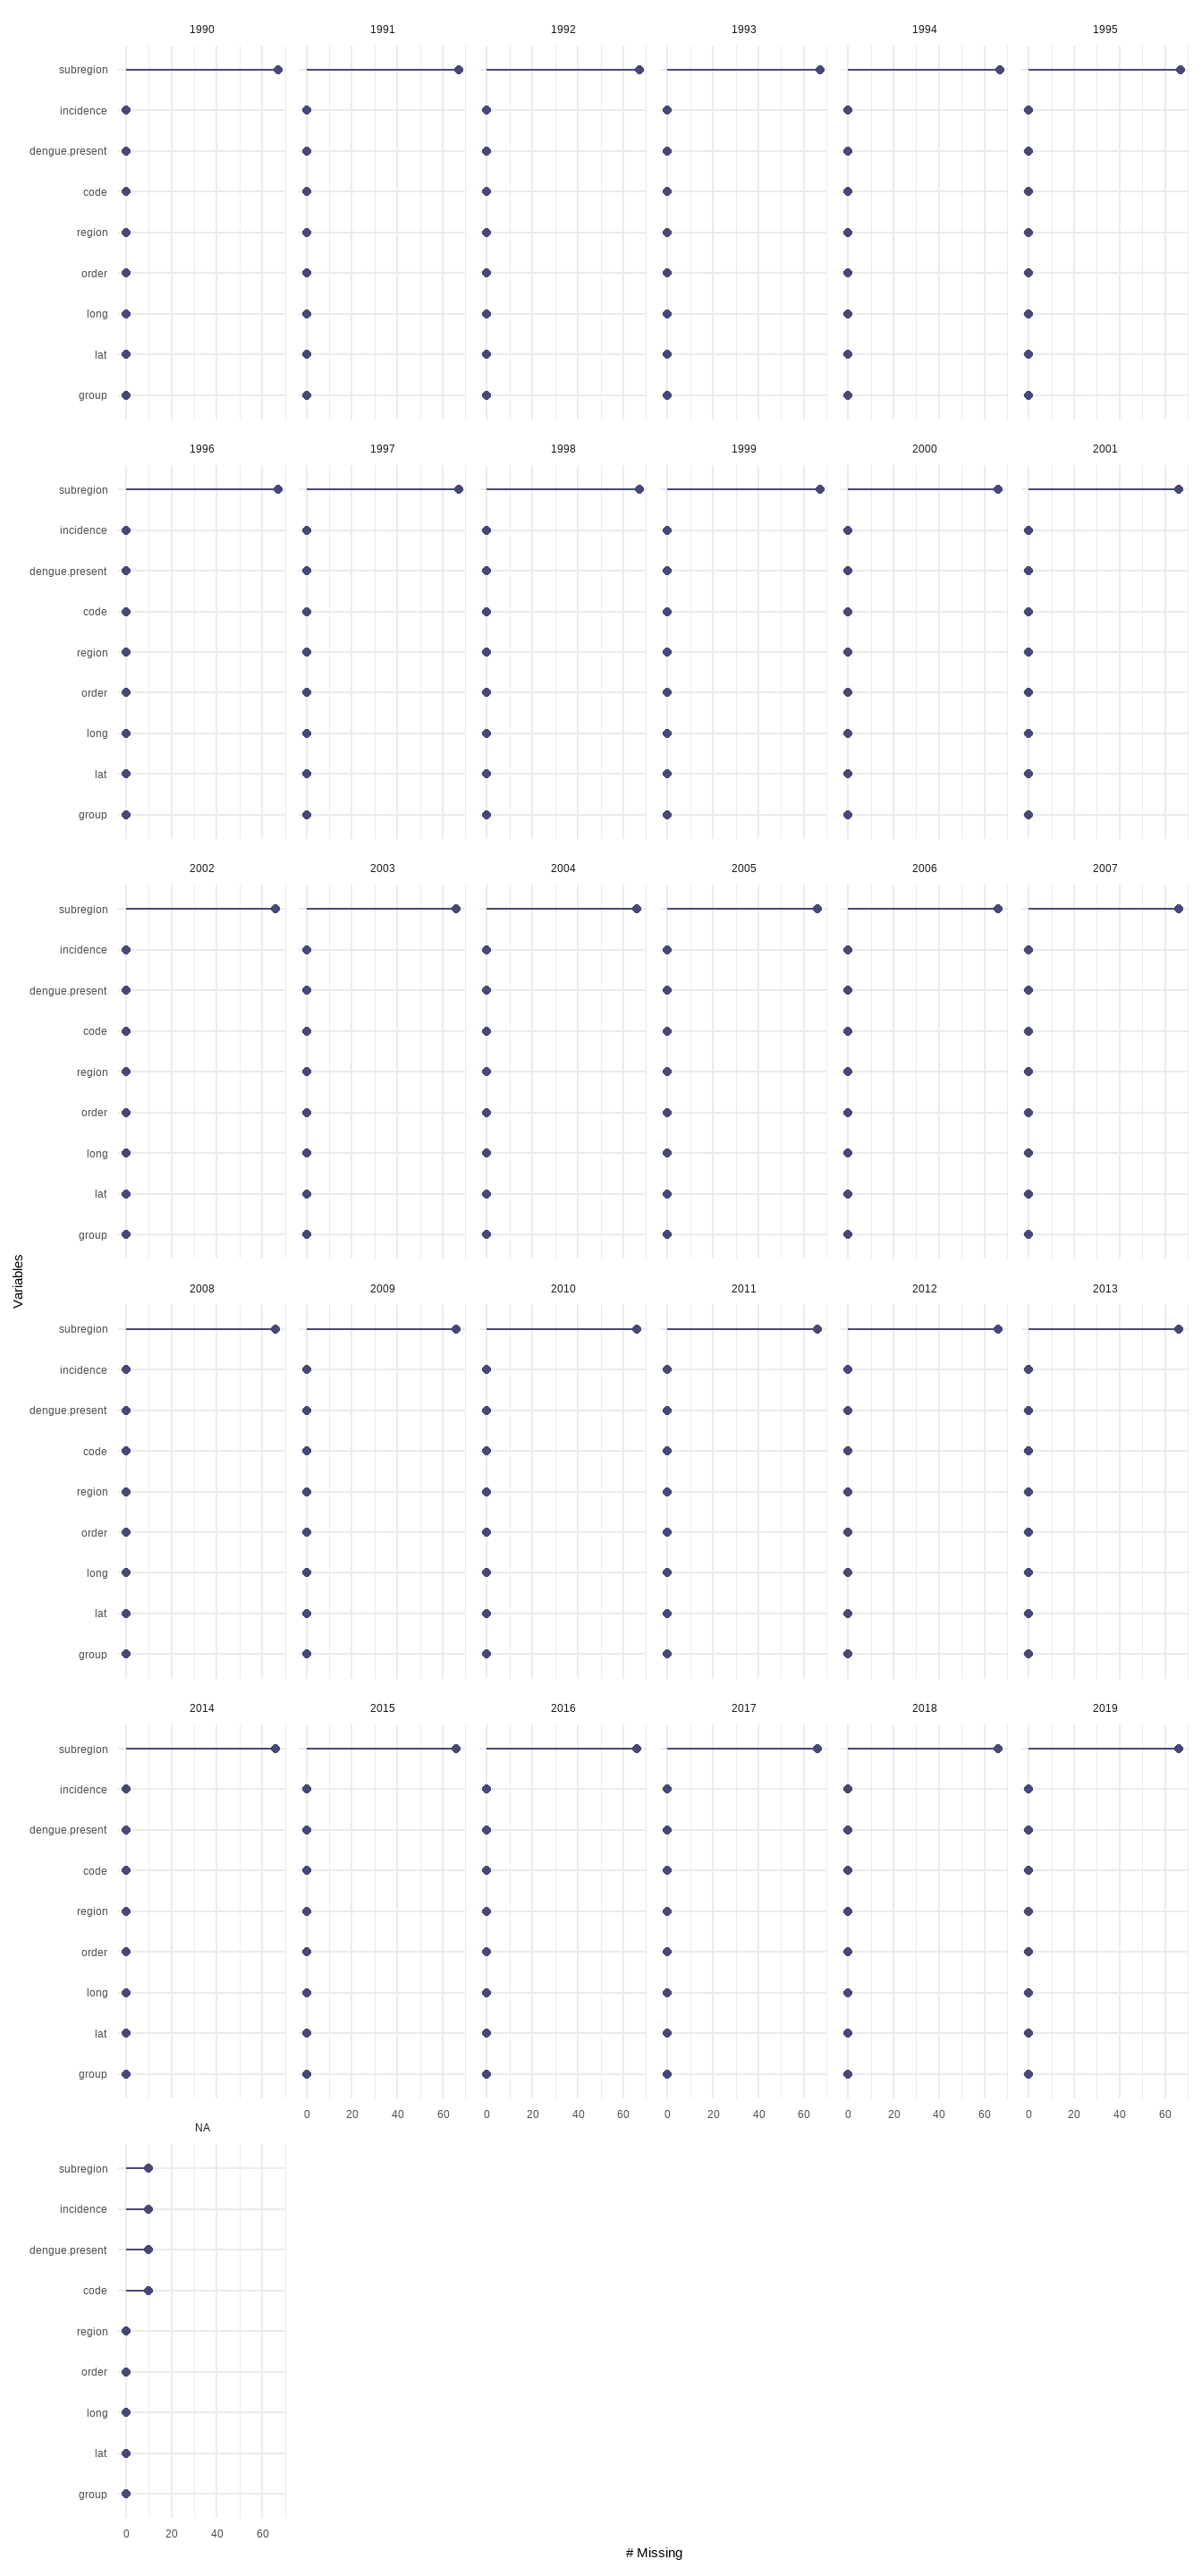
\includegraphics{ch2_files/figure-pdf/unnamed-chunk-30-1.pdf}

\section{Explore Missing
Relationships}\label{explore-missing-relationships}

\subsection{\texorpdfstring{\texttt{denguedatahub::srilanka\_weekly\_data}}{denguedatahub::srilanka\_weekly\_data}}\label{denguedatahubsrilanka_weekly_data-4}

R
Code:\ldots\ldots\ldots\ldots\ldots\ldots\ldots\ldots\ldots\ldots\ldots.

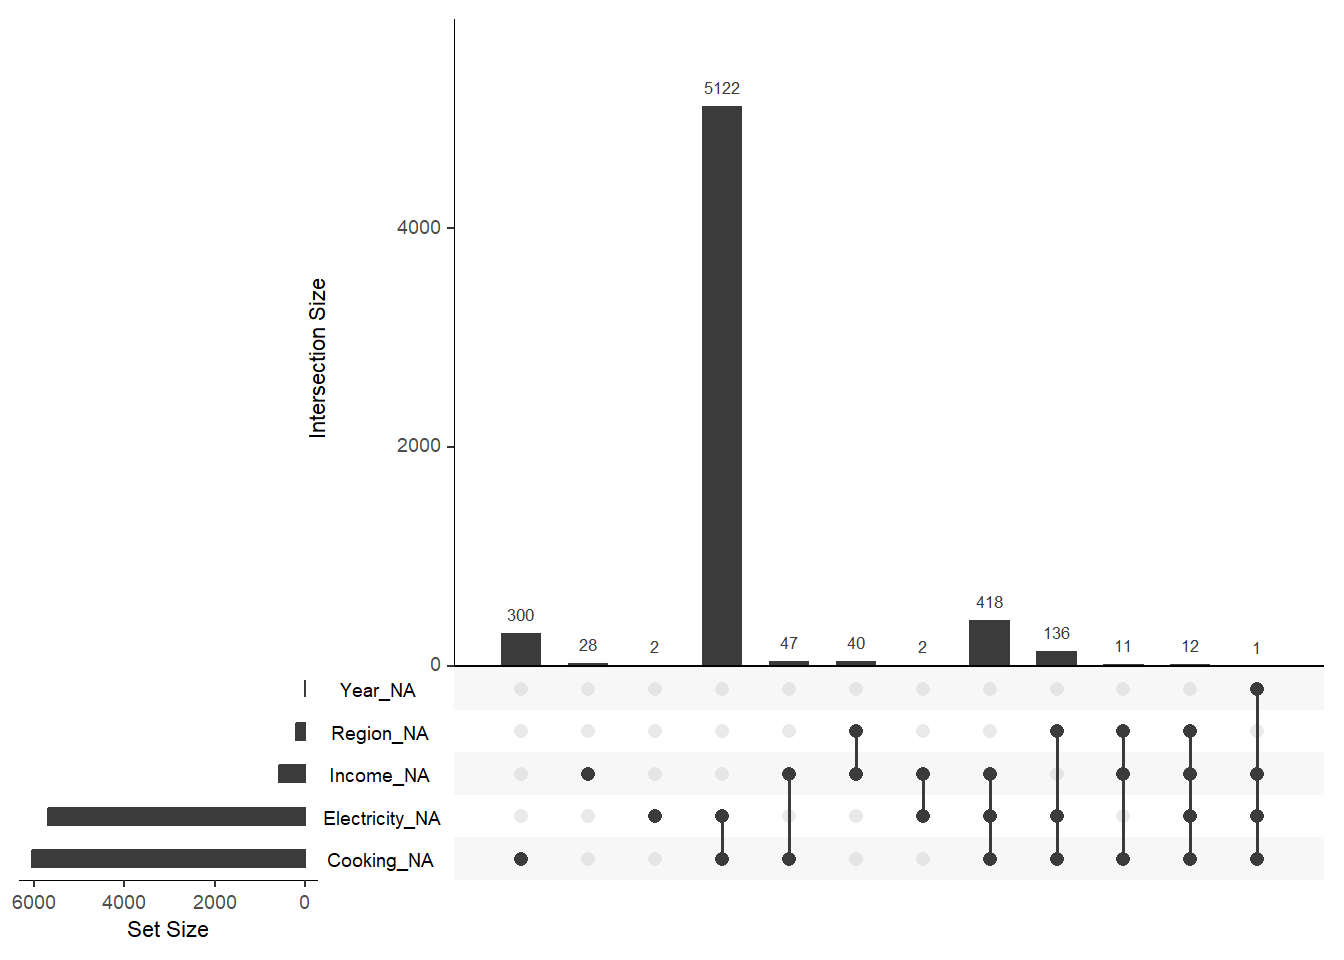
\includegraphics{ch2_files/figure-pdf/unnamed-chunk-31-1.pdf}

\subsection{\texorpdfstring{\texttt{drone::worldbankdata}}{drone::worldbankdata}}\label{droneworldbankdata}

\begin{Shaded}
\begin{Highlighting}[]
\CommentTok{\# install.packages("devtools")}
\NormalTok{devtools}\SpecialCharTok{::}\FunctionTok{install\_github}\NormalTok{(}\StringTok{"thiyangt/drone"}\NormalTok{)}
\end{Highlighting}
\end{Shaded}

\begin{Shaded}
\begin{Highlighting}[]
\FunctionTok{library}\NormalTok{(tibble)}
\FunctionTok{library}\NormalTok{(drone)}
\FunctionTok{data}\NormalTok{(}\StringTok{"worldbankdata"}\NormalTok{)}
\NormalTok{worldbankdata}
\end{Highlighting}
\end{Shaded}

\begin{verbatim}
# A tibble: 7,937 x 7
   Country Code  Region                     Year Cooking Electricity Income
   <fct>   <fct> <fct>                     <dbl>   <dbl>       <dbl> <fct> 
 1 Aruba   ABW   Latin America & Caribbean  1990      NA       100   H     
 2 Aruba   ABW   Latin America & Caribbean  2000      NA        91.7 H     
 3 Aruba   ABW   Latin America & Caribbean  2013      NA       100   H     
 4 Aruba   ABW   Latin America & Caribbean  2014      NA       100   H     
 5 Aruba   ABW   Latin America & Caribbean  2015      NA       100   H     
 6 Aruba   ABW   Latin America & Caribbean  2016      NA       100   H     
 7 Aruba   ABW   Latin America & Caribbean  2017      NA       100   H     
 8 Aruba   ABW   Latin America & Caribbean  2018      NA       100   H     
 9 Aruba   ABW   Latin America & Caribbean  2019      NA       100   H     
10 Aruba   ABW   Latin America & Caribbean  2020      NA       100   H     
# i 7,927 more rows
\end{verbatim}

\begin{quote}
Your turn: Perform a data profiling analysis on \texttt{worldbankdata}.
\end{quote}

\begin{Shaded}
\begin{Highlighting}[]
\NormalTok{worldbankdata }\SpecialCharTok{|\textgreater{}}
  \FunctionTok{as\_shadow\_upset}\NormalTok{() }\SpecialCharTok{|\textgreater{}}
\NormalTok{  UpSetR}\SpecialCharTok{::}\FunctionTok{upset}\NormalTok{()}
\end{Highlighting}
\end{Shaded}

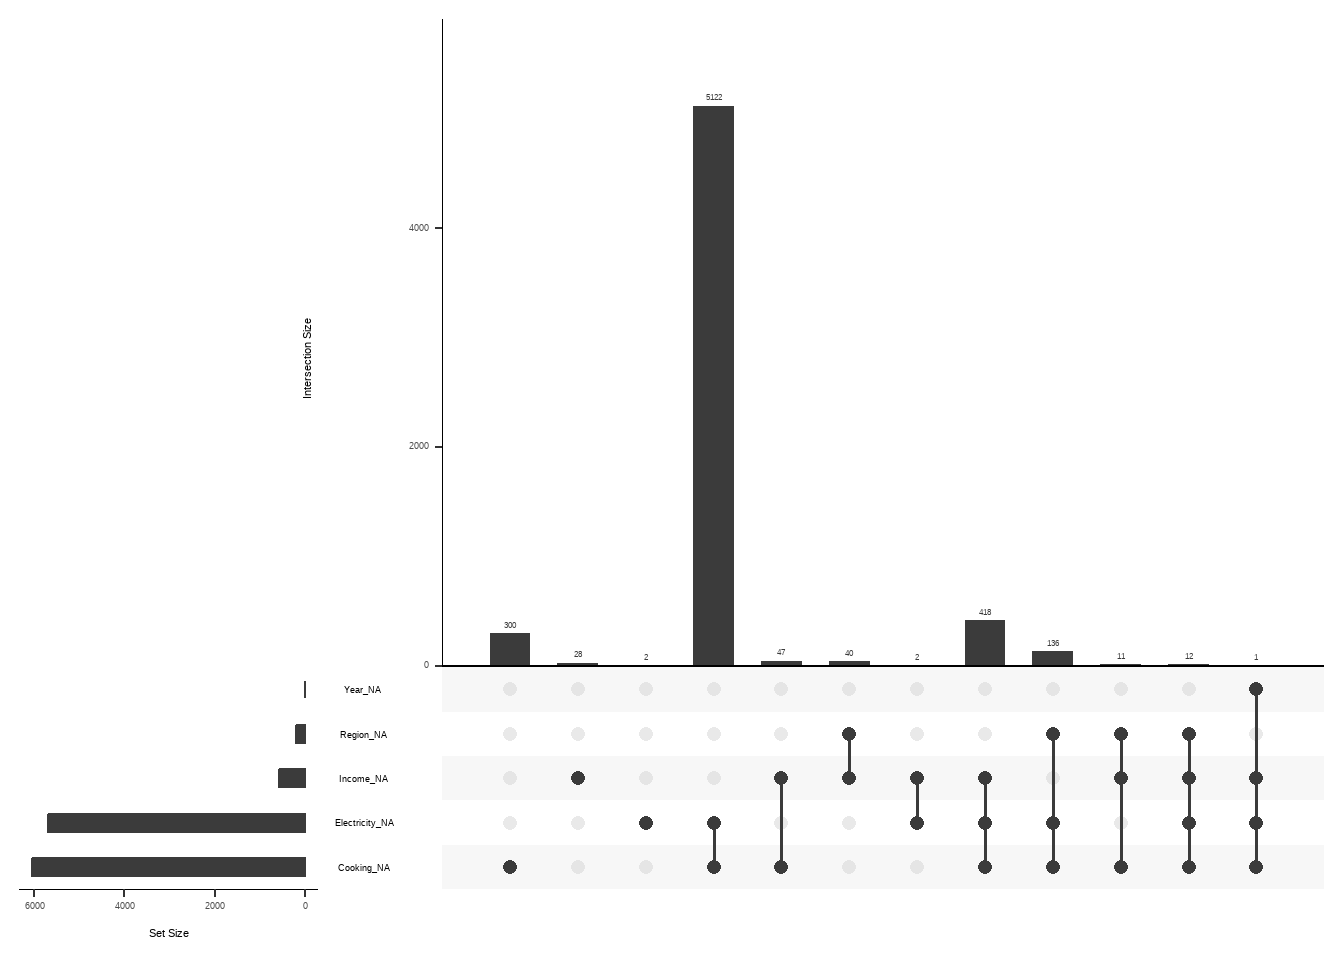
\includegraphics{ch2_files/figure-pdf/unnamed-chunk-34-1.pdf}

\section{Visualizing Values That Meet Specific
Conditions}\label{visualizing-values-that-meet-specific-conditions}

Visualize values greater than 50 in the cases Column of the
\texttt{srilanka\_weekly\_data} dataset.

R
Code:\ldots\ldots\ldots\ldots\ldots\ldots\ldots\ldots\ldots\ldots\ldots.

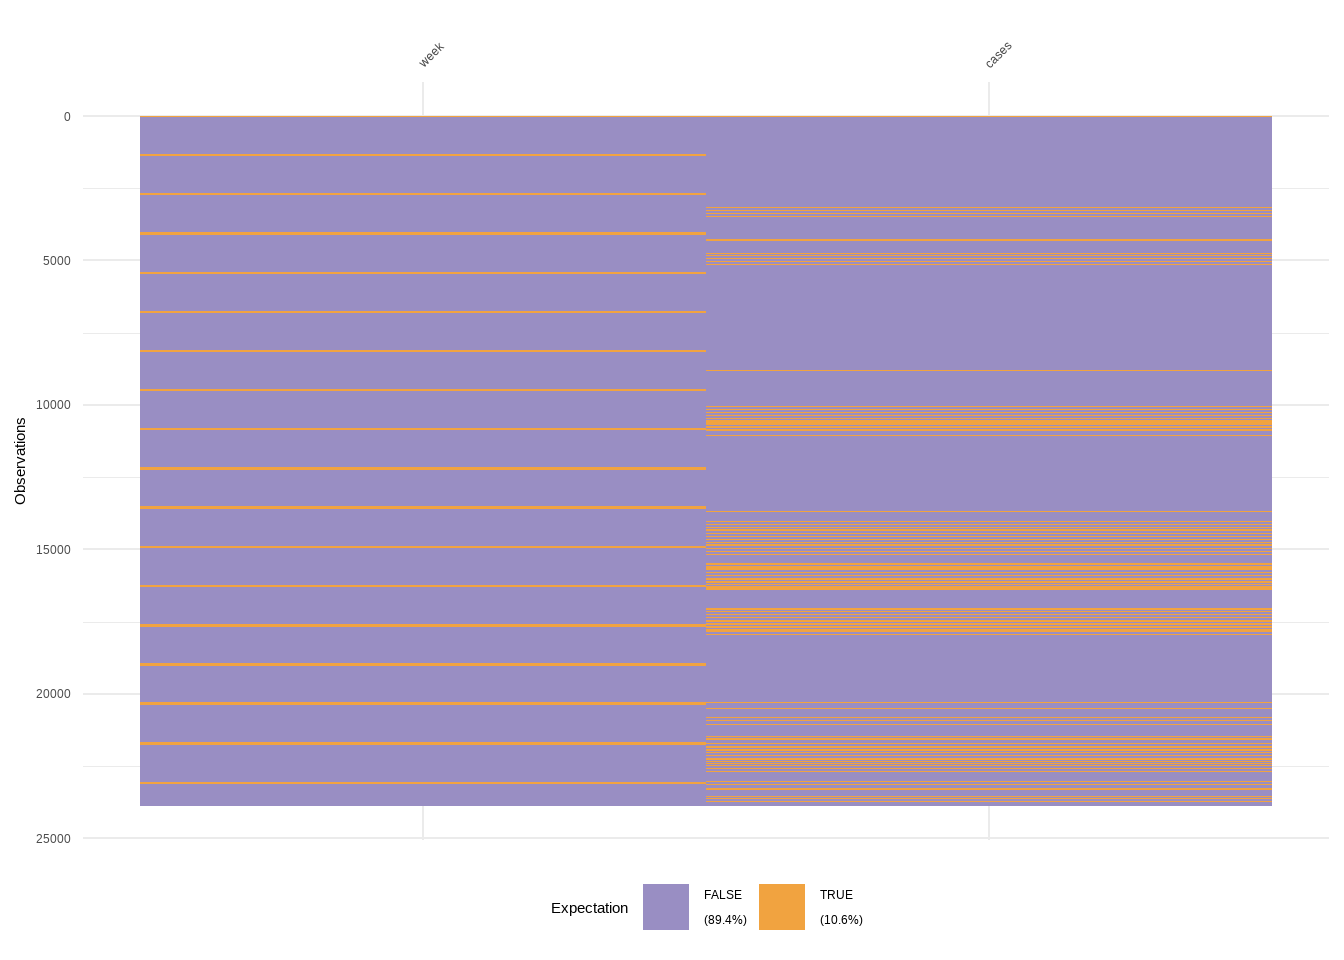
\includegraphics{ch2_files/figure-pdf/unnamed-chunk-35-1.pdf}

\section{Descriptive Statistcs}\label{descriptive-statistcs}

\subsection{denguedatahub::srilanka\_weekly\_data}\label{denguedatahubsrilanka_weekly_data-5}

R
Code:\ldots\ldots\ldots\ldots\ldots\ldots\ldots\ldots\ldots\ldots\ldots.

\begin{Shaded}
\begin{Highlighting}[]
\FunctionTok{describe}\NormalTok{(srilanka\_weekly\_data)}
\end{Highlighting}
\end{Shaded}

\begin{verbatim}
# A tibble: 3 x 26
  described_variables     n    na   mean    sd se_mean   IQR skewness kurtosis
  <chr>               <int> <int>  <dbl> <dbl>   <dbl> <dbl>    <dbl>    <dbl>
1 year                23882     0 2015.   5.09  0.0329     9  0.00661    -1.20
2 week                23882     0   26.3 15.1   0.0974    26  0.0323     -1.19
3 cases               23882     0   31.2 82.0   0.531     26 10.3       190.  
# i 17 more variables: p00 <dbl>, p01 <dbl>, p05 <dbl>, p10 <dbl>, p20 <dbl>,
#   p25 <dbl>, p30 <dbl>, p40 <dbl>, p50 <dbl>, p60 <dbl>, p70 <dbl>,
#   p75 <dbl>, p80 <dbl>, p90 <dbl>, p95 <dbl>, p99 <dbl>, p100 <dbl>
\end{verbatim}

\subsection{denguedatahub::worldbankdata}\label{denguedatahubworldbankdata}

R
Code:\ldots\ldots\ldots\ldots\ldots\ldots\ldots\ldots\ldots\ldots\ldots.

\begin{Shaded}
\begin{Highlighting}[]
\FunctionTok{describe}\NormalTok{(worldbankdata)}
\end{Highlighting}
\end{Shaded}

\begin{verbatim}
# A tibble: 3 x 26
  described_variables     n    na   mean    sd se_mean   IQR skewness kurtosis
  <chr>               <int> <int>  <dbl> <dbl>   <dbl> <dbl>    <dbl>    <dbl>
1 Year                 7936     1 2005.   10.4   0.117  18    -0.0123    -1.21
2 Cooking              1890  6047   65.5  38.5   0.885  72.7  -0.612     -1.31
3 Electricity          2244  5693   84.4  26.5   0.558  20.1  -1.63       1.32
# i 17 more variables: p00 <dbl>, p01 <dbl>, p05 <dbl>, p10 <dbl>, p20 <dbl>,
#   p25 <dbl>, p30 <dbl>, p40 <dbl>, p50 <dbl>, p60 <dbl>, p70 <dbl>,
#   p75 <dbl>, p80 <dbl>, p90 <dbl>, p95 <dbl>, p99 <dbl>, p100 <dbl>
\end{verbatim}

\section{Diagnosing outliers}\label{diagnosing-outliers}

\subsection{denguedatahub::srilanka\_weekly\_data}\label{denguedatahubsrilanka_weekly_data-6}

R
Code:\ldots\ldots\ldots\ldots\ldots\ldots\ldots\ldots\ldots\ldots\ldots.

\begin{verbatim}
# A tibble: 3 x 6
  variables outliers_cnt outliers_ratio outliers_mean with_mean without_mean
  <chr>            <int>          <dbl>         <dbl>     <dbl>        <dbl>
1 year                 0            0            NaN     2015.        2015. 
2 week                 0            0            NaN       26.3         26.3
3 cases             2617           11.0          181.      31.2         12.8
\end{verbatim}

\subsection{denguedatahub::worldbankdata}\label{denguedatahubworldbankdata-1}

R
Code:\ldots\ldots\ldots\ldots\ldots\ldots\ldots\ldots\ldots\ldots\ldots.

\begin{verbatim}
# A tibble: 3 x 6
  variables   outliers_cnt outliers_ratio outliers_mean with_mean without_mean
  <chr>              <int>          <dbl>         <dbl>     <dbl>        <dbl>
1 Year                   0           0            NaN      2005.        2005. 
2 Cooking                0           0            NaN        65.5         65.5
3 Electricity          330           4.16          28.1      84.4         94.1
\end{verbatim}

\section{Bi-variate relationships}\label{bi-variate-relationships}

\subsection{drone::worldbankdata}\label{droneworldbankdata-1}

R
Code:\ldots\ldots\ldots\ldots\ldots\ldots\ldots\ldots\ldots\ldots\ldots.

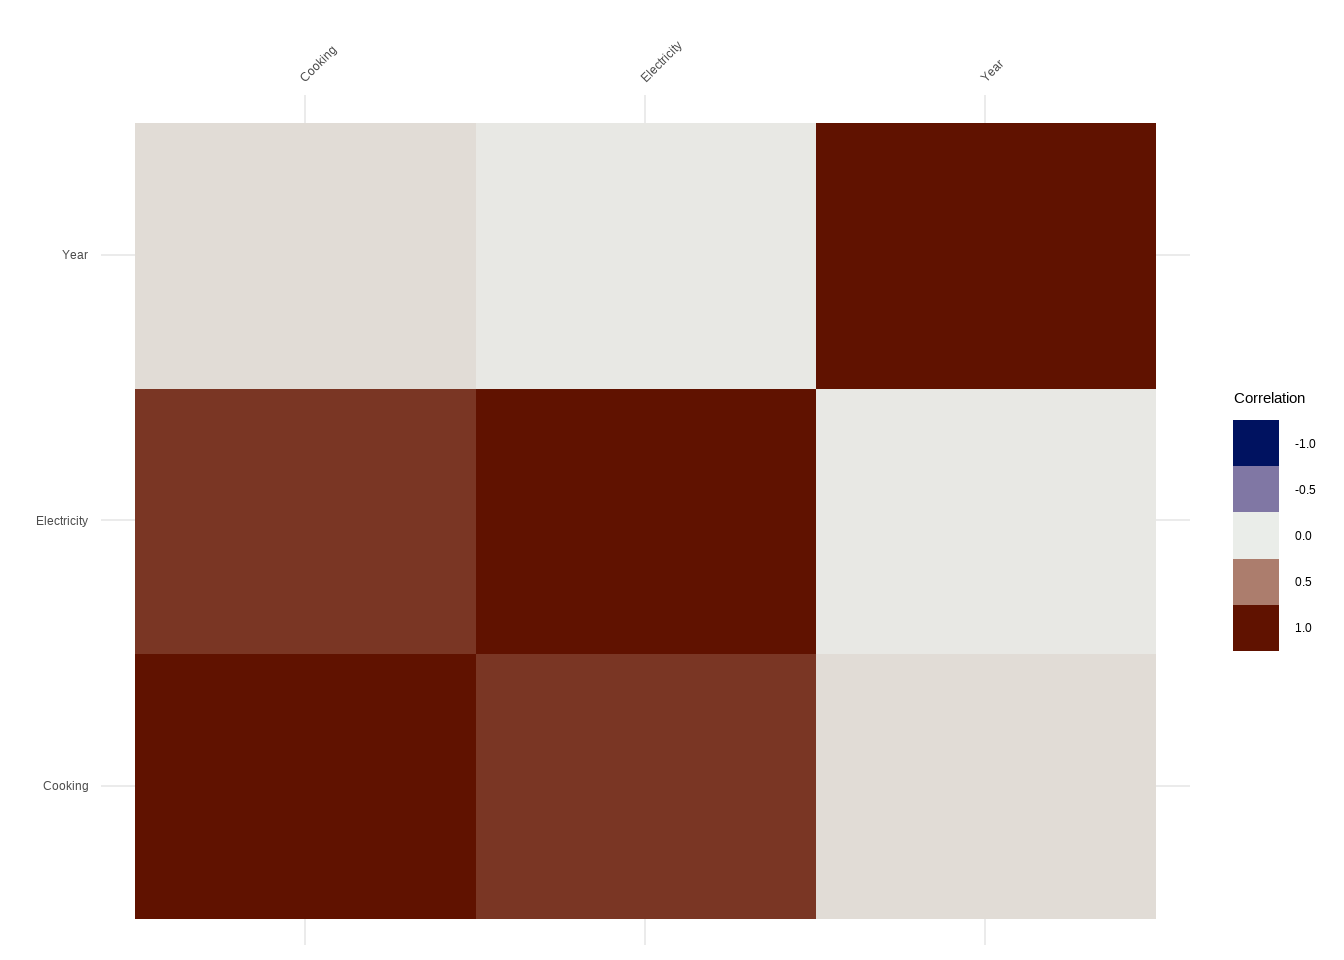
\includegraphics{ch2_files/figure-pdf/unnamed-chunk-40-1.pdf}

\section{Exercise}\label{exercise-1}

\begin{enumerate}
\def\labelenumi{\arabic{enumi}.}
\item
  Explore the methodologies behind each code used to generate the
  outputs.
\item
  Explore data validation methods implemented in R.
\item
  Perform data quality analysis for the following datasets and properly
  report your findings:
\end{enumerate}

\begin{itemize}
\item
  Datasets in the denguedatahub package in R
\item
  Datasets in the drone package in R
\item
  The penguins dataset in the palmerpenguins package in R
\end{itemize}

\begin{enumerate}
\def\labelenumi{\arabic{enumi}.}
\setcounter{enumi}{3}
\tightlist
\item
  Perform a data quality analysis on the following data set.
\end{enumerate}

\begin{Shaded}
\begin{Highlighting}[]
\FunctionTok{library}\NormalTok{(DSjobtracker)}
\FunctionTok{data}\NormalTok{(DSraw)}
\end{Highlighting}
\end{Shaded}

\bookmarksetup{startatroot}

\chapter{Techniques for Addressing Data Quality
Issues}\label{techniques-for-addressing-data-quality-issues}

\section{Assignment: 20 Marks}\label{assignment-20-marks}

\subsection{Instructions}\label{instructions}

\begin{itemize}
\item
  Organize into groups, with a maximum of 5 members per group.
\item
  Each member should have a distinct role and individual contribution
  toward the final submission.
\end{itemize}

\subsection{Task}\label{task}

\begin{itemize}
\item
  Identify and explore methods to address common data quality issues
  (e.g., handling missing values, detecting and managing outliers,
  resolving data inconsistencies, etc.).
\item
  Use a sample dataset to demonstrate these methods in R. Your
  implementation should include clear R code and explanations of the
  methodologies used.
\end{itemize}

\subsection{Submission Requirements}\label{submission-requirements}

\textbf{1. Report:} The group must prepare a comprehensive report that
details:

\begin{itemize}
\item
  An overview of data quality issues and the chosen methods.
\item
  The step-by-step process for implementing these methods in R.
\item
  Sample R code with commentary and explanations. Insights or findings
  based on the sample dataset.
\end{itemize}

\textbf{2. Presentation:}

\begin{itemize}
\tightlist
\item
  Each member must present only the part of the work they personally
  contributed to.
\end{itemize}

\subsection{Evaluation Criteria}\label{evaluation-criteria}

\begin{itemize}
\item
  Quality and accuracy of the report, including clarity of explanations
  and code functionality. Effectiveness and relevance of the techniques
  chosen for data quality issues.
\item
  Depth of individual contributions in both the report and the
  presentation.
\item
  Cohesiveness and clarity of the group presentation.
\item
  To earn marks, each member must contribute to both the written report
  and the presentation.
\end{itemize}

\subsection{Deadline}\label{deadline}

\begin{itemize}
\item
  Submit the report and presentation files by November 9, 2024
\item
  Final presentations: November \textsubscript{10} 12, 2024
\end{itemize}

\bookmarksetup{startatroot}

\chapter{Types of Consultancy
Projects}\label{types-of-consultancy-projects}

\section{Common Types of Consultancy
Projects}\label{common-types-of-consultancy-projects}

\begin{enumerate}
\def\labelenumi{\arabic{enumi}.}
\item
  Client-Provided Data Analysis
\item
  Data Collection and Analysis (designs a data collection strategy,
  gathers data)
\item
  Experimental Design and Analysis
\item
  Model Development and Validation
\item
  Quality Control and Process Improvement
\item
  Survey Design and Analysis
\item
  Data Visualization and Reporting
\item
  Predictive Analytics and Forecasting
\item
  Statistical Software Implementation and Training
\item
  Training and workshops
\end{enumerate}

\section{Exercise}\label{exercise-2}

Discuss the differences among various types of consultancy projects,
highlighting the role of clients and providing examples.

\bookmarksetup{startatroot}

\chapter{Verbal Communication}\label{verbal-communication}

\section{Active Listening}\label{active-listening}

\begin{itemize}
\item
  Active listening is a key communication skill.
\item
  Active listening is about understanding the speaker's message and
  responding to them.
\item
  Active listening includes verbal and non-verbal cues.
\end{itemize}

\section{Active Listening: Key
Components}\label{active-listening-key-components}

In what ways can you show that you are listening actively?

\section{Benefits of Active Listening for a Smooth Consultancy
Session}\label{benefits-of-active-listening-for-a-smooth-consultancy-session}

How active listening benefits statistical consultancy?

\section{Asking Questions}\label{asking-questions}

\begin{enumerate}
\def\labelenumi{\arabic{enumi}.}
\item
  Plan what information do we need?
\item
  Listen carefully
\item
  Slow down
\item
  Clarify all terms
\item
  Ask if you do not understand
\item
  Take notes
\end{enumerate}

\section{Common questions}\label{common-questions}

\begin{enumerate}
\def\labelenumi{\arabic{enumi}.}
\item
  Research area/ domain
\item
  Goals and objectives
\item
  Motivation
\item
  Significance of the study
\item
  Novelty of the study topic
\item
  Related work (literature, relevant methods, etc)
\item
  Data collection procedure
\item
  Sample size
\item
  Structure of data
\item
  Missing values, outliers
\item
  Limitations of data
\item
  Survey/ Census: Target population, variables, sampling design,
  sampling frame, sources of bias, sampling unit
\item
  Design of experiments: experimental unit, sampling unit, factors,
  treatments, responses, randomization, blocking, design
\item
  Background reading
\end{enumerate}

\section{Client Question Checklist}\label{client-question-checklist}

Create a Checklist for Reviewing Client Information Before Starting
Analysis?

\section{Question types}\label{question-types}

\subsection{Close probe questions (usually with Yes or
No)}\label{close-probe-questions-usually-with-yes-or-no}

\begin{itemize}
\item
  Did you interview every person on the list?
\item
  Are there any missing values?
\end{itemize}

\subsection{Open probes (long
responses)}\label{open-probes-long-responses}

\begin{itemize}
\item
  What factors are likely to affect the response?
\item
  I'd like to hear more about the independent variables you plan to
  measure.
\item
  Is there anything more that we should discuss related to food
  packaging types before we go on to discuss the variables you plan to
  measure?
\end{itemize}

\subsection{Specific questions}\label{specific-questions}

\begin{itemize}
\item
  What is the sample size?
\item
  When did you collect this data?
\item
  Which methodology did you use for this analysis?
\end{itemize}

\section{Cognitive Load Theory: Forms of Cognitive
Load}\label{cognitive-load-theory-forms-of-cognitive-load}

\begin{enumerate}
\def\labelenumi{\arabic{enumi}.}
\item
  Intrinsic cognitive load
\item
  Extraneous cognitive load
\item
  Germane cognitive load
\end{enumerate}

\section{Ask if you don't understand}\label{ask-if-you-dont-understand}

Restate factual information and make sure you have gotten everything
correct.

\begin{itemize}
\item
  Let me make sure that I understand \ldots{}
\item
  Do I have this correctly?
\item
  So a sampling unit is an individual person, is that correct?
\end{itemize}

\bookmarksetup{startatroot}

\chapter{Written Communication}\label{written-communication}

\section{Components of a statistical consultancy
report}\label{components-of-a-statistical-consultancy-report}

\begin{enumerate}
\def\labelenumi{\arabic{enumi}.}
\item
  Cover page

  \begin{itemize}
  \item
    Title of the Report
  \item
    Client's Name and Contact Information
  \item
    Consultant's Name and Contact Information
  \item
    Date of Submission
  \item
    Confidentiality Statement (if applicable)
  \end{itemize}
\item
  Introduction

  \begin{itemize}
  \item
    Background information
  \item
    Objectives
  \item
    Scope
  \end{itemize}
\item
  Methodology
\item
  Results
\item
  Discussion
\item
  Conclusions
\item
  Appendices
\item
  References
\end{enumerate}

\section{Exercise}\label{exercise-3}

What are the differences between a statistical consultancy report, a
thesis, and a journal article?

\section{Other essential documents commonly needed in statistical
consultancy}\label{other-essential-documents-commonly-needed-in-statistical-consultancy}

\begin{enumerate}
\def\labelenumi{\arabic{enumi}.}
\item
  Log book
\item
  Meeting minutes
\item
  Letter head
\item
  Project plan
\item
  Data collection plan
\item
  Progress report
\item
  Technical documentation
\item
  Follow up documents
\item
  Final report
\item
  Presentation
\end{enumerate}

These documents help maintain clear communication, ensure
accountability, and provide a record of the consultancy's progression
and outcomes.

\bookmarksetup{startatroot}

\chapter{Writing Manuscript}\label{writing-manuscript}

\bookmarksetup{startatroot}

\chapter{Abstract}\label{abstract}

\section{Role of abstract}\label{role-of-abstract}

\begin{enumerate}
\def\labelenumi{\arabic{enumi}.}
\item
  Grab attention
\item
  Establishes Relevance: decide whether to continue reading
\item
  Gives an idea of the quality of the work
\item
  Serves as a marketing tool
\item
  Making the paper discoverabl
\end{enumerate}

\section{Types of abstracts}\label{types-of-abstracts}

\begin{enumerate}
\def\labelenumi{\arabic{enumi}.}
\item
  Descriptive abstract
\item
  Informative abstract
\item
  Critical abstract
\item
  Structured abstract
\item
  Graphical abstract
\item
  Highlight abstract
\end{enumerate}

\section{How to write an abstract?}\label{how-to-write-an-abstract}

Your abstract should answer the following questions.

\begin{enumerate}
\def\labelenumi{\arabic{enumi}.}
\item
  What did you do?
\item
  Why did you do?
\item
  How did you do?
\item
  What did you find?
\item
  What do your findings mean?
\item
  What are the advantages of your findings?
\item
  How well does it work?
\end{enumerate}

\section{Features of a good abstract}\label{features-of-a-good-abstract}

\begin{enumerate}
\def\labelenumi{\arabic{enumi}.}
\item
  Stands on its own
\item
  Avoid ``I'', ``We''
\item
  Avoid trade names, acronyms, abbreviations, or symbols
\item
  Use active voice instead of passive voice (the study tested rather
  than it was tested by the study)
\end{enumerate}

\bookmarksetup{startatroot}

\chapter{Introduction}\label{introduction}

\begin{enumerate}
\def\labelenumi{\arabic{enumi}.}
\item
  Introduce general topic
\item
  Past studies
\item
  Highlight the gap
\item
  Objectives of the current study
\end{enumerate}

\bookmarksetup{startatroot}

\chapter{Guidelines on how to divide paragraphs in the
introduction}\label{guidelines-on-how-to-divide-paragraphs-in-the-introduction}

In class discussion with examples

1\ldots\ldots\ldots\ldots..

2\ldots\ldots\ldots\ldots..

3\ldots\ldots\ldots\ldots..

4\ldots\ldots\ldots\ldots..

5\ldots\ldots\ldots\ldots..

6\ldots\ldots\ldots\ldots..

7\ldots\ldots\ldots\ldots..

\begin{enumerate}
\def\labelenumi{\arabic{enumi}.}
\setcounter{enumi}{7}
\tightlist
\item
  Significance of your study
\end{enumerate}

8.1\ldots\ldots\ldots\ldots\ldots\ldots{}

8.2\ldots\ldots\ldots\ldots\ldots\ldots{}

8.3\ldots\ldots\ldots\ldots\ldots\ldots{}

\bookmarksetup{startatroot}

\chapter{Literature review}\label{literature-review}

\begin{itemize}
\item
  Chronological
\item
  Thematic
\item
  Methodological
\end{itemize}

\bookmarksetup{startatroot}

\chapter{Methodology}\label{methodology}

\begin{itemize}
\tightlist
\item
  How the research was conducted
\end{itemize}

\bookmarksetup{startatroot}

\chapter{Results}\label{results}

\begin{itemize}
\tightlist
\item
  What you discovered through your research
\end{itemize}

\bookmarksetup{startatroot}

\chapter{Conclusions and Discussions}\label{conclusions-and-discussions}

\begin{itemize}
\item
  Interpret the results
\item
  Explain their implications
\item
  Address unexpected findings
\item
  Limitations in your study
\item
  Future directions
\end{itemize}

\bookmarksetup{startatroot}

\chapter{Other sections}\label{other-sections}

\begin{itemize}
\item
  References
\item
  Acknowledgement
\end{itemize}

\bookmarksetup{startatroot}

\chapter{Research misconducts}\label{research-misconducts}

\begin{itemize}
\item
  Data falsification
\item
  Data fabrication
\item
  Plagiarism
\end{itemize}

\bookmarksetup{startatroot}

\chapter{Handling misconduct}\label{handling-misconduct}

\begin{itemize}
\item
  Rejection
\item
  Retraction
\end{itemize}

\bookmarksetup{startatroot}

\chapter*{References}\label{references}
\addcontentsline{toc}{chapter}{References}

\markboth{References}{References}

\phantomsection\label{refs}
\begin{CSLReferences}{0}{1}
\end{CSLReferences}




\end{document}
